%===============================================================================
% LaTeX sjabloon voor de bachelorproef toegepaste informatica aan HOGENT
% Meer info op https://github.com/HoGentTIN/latex-hogent-report
%===============================================================================

\documentclass[dutch,dit,thesis]{hogentreport}

% TODO:
% - If necessary, replace the option `dit`' with your own department!
%   Valid entries are dbo, dbt, dgz, dit, dlo, dog, dsa, soa
% - If you write your thesis in English (remark: only possible after getting
%   explicit approval!), remove the option "dutch," or replace with "english".

\usepackage{lipsum} % For blind text, can be removed after adding actual content
\usepackage{listings}
\lstdefinestyle{PowerShellStyle}{
    language=PowerShell,
    basicstyle=\small\ttfamily,
    keywordstyle=\bfseries\color{blue},
    stringstyle=\color{orange},
    commentstyle=\color{green},
    showstringspaces=false,
    numbers=left,
    numberstyle=\tiny,
    numbersep=5pt,
    frame=single,
    breaklines=true,
    breakatwhitespace=true,
    tabsize=4
}
\lstdefinelanguage{PowerShell}{
    morekeywords={Add-Content, Add-History, Add-Member, Add-PSSnapin, Clear-Content, Clear-History, Clear-Item, Clear-ItemProperty, Clear-Variable, Compare-Object, Complete-Transaction, Connect-PSSession, ConvertFrom-Json, Convert-Path, ConvertTo-Html, ConvertTo-Json, Copy-Item, Copy-ItemProperty, Debug-Process, Disable-PSBreakpoint, Disable-PSRemoting, Disable-PSSessionConfiguration, Enable-PSBreakpoint, Enable-PSRemoting, Enable-PSSessionConfiguration, Enter-PSSession, Exit-PSSession, Export-Alias, Export-Csv, Export-PSSession, ForEach-Object, Format-Table, Get-Acl, Get-Alias, Get-AuthenticodeSignature, Get-ChildItem, Get-Command, Get-ComputerInfo, Get-Content, Get-Credential, Get-Culture, Get-Date, Get-Event, Get-EventLog, Get-ExecutionPolicy, Get-History, Get-Host, Get-Item, Get-ItemProperty, Get-Job, Get-Location, Get-Member, Get-Module, Get-NetAdapter, Get-NetIPAddress, Get-NetIPConfiguration, Get-Process, Get-PSBreakpoint, Get-PSDrive, Get-PSProvider, Get-PSSession, Get-PSSessionConfiguration, Get-PSSnapin, Get-Service, Get-TimeZone, Get-Transaction, Get-UICulture, Get-Unique, Get-Variable, Get-WinEvent, Get-WmiObject, Group-Object, Import-Alias, Import-Csv, Import-PSSession, Invoke-Command, Invoke-Expression, Invoke-History, Invoke-Item, Invoke-RestMethod, Invoke-WebRequest, Join-Path, Measure-Command, Measure-Object, Move-Item, New-Event, New-Item, New-ItemProperty, New-Object, New-PSDrive, New-Service, New-TimeSpan, New-Variable, Out-Default, Out-File, Out-GridView, Out-Host, Out-Null, Out-Printer, Out-String, Pop-Location, Push-Location, Read-Host, Remove-Acl, Remove-Event, Remove-Item, Remove-ItemProperty, Remove-Job, Remove-Module, Remove-PSBreakpoint, Remove-PSDrive, Remove-PSProvider, Remove-PSSession, Remove-PSSnapin, Remove-Service, Remove-Variable, Rename-Item, Rename-ItemProperty, Resolve-Path, Restart-Service, Resume-Service, Select-Object, Select-String, Set-Acl, Set-Alias, Set-AuthenticodeSignature, Set-Content, Set-Date, Set-ExecutionPolicy, Set-Item, Set-ItemProperty, Set-Location, Set-NetIPAddress, Set-Service, Set-TimeZone, Set-Variable, Sort-Object, Split-Path, Start-Job, Start-Process, Start-Service, Start-Sleep, Start-Transaction, Stop-Computer, Stop-Job, Stop-Process, Stop-Service, Stop-Transcript, Suspend-Service, Tee-Object, Test-Connection, Test-Path, Update-Help, Update-TypeData, Where-Object, Write-Debug, Write-Error, Write-Host, Write-Output, Write-Progress, Write-Verbose, Write-Warning},
    sensitive=true,
    morecomment=[l]}
    
\lstdefinelanguage{LinuxCommands}{
    % Definieer de kleuren voor de verschillende elementen
    keywordstyle=\color{blue}\bfseries,  % Sleutelwoorden (bijv. cd, ls)
    commentstyle=\color{gray}\textit,    % Opmerkingen (beginnend met #)
    stringstyle=\color{red},             % Strings (bijv. "Hello World")
    % Specificeer de lijst met sleutelwoorden
    keywords={cd, ls, pwd, echo, cat, rm, mv, cp},
    % Schakel in dat spaties in strings behouden blijven
    keepspaces=true,
    % Stel de basisinstellingen in
    basicstyle=\ttfamily\small,         % Het lettertype en de grootte
    columns=fullflexible,               % De breedte van de tekens
    % Voeg een lijnnummers toe aan de code
    numbers=left,
    numbersep=5pt,
    numberstyle=\tiny\color{gray},
    % Voeg een lijst met opties toe aan de stijl
    xleftmargin=0.5cm,
    frame=tb,
    framesep=4pt,
    framerule=0pt,
    % Stel de tabgrootte in op 4 tekens
    tabsize=4,
    % Schakel in dat regelonderbrekingen toegestaan zijn
    breaklines=true,
    breakatwhitespace=true,
}
\lstdefinestyle{customStyleBashDark}{
    language=Bash,
    numbers=left,%position of line numbers (left/right/none, i.e. no line numbers)
    basicstyle=\footnotesize\ttfamily\color[RGB]{255,255,255},%font size/family/etc. for source (e.g. basicstyle=\ttfamily\small)
    numberstyle=\color[RGB]{0,0,0},%style used for line-numbers
    backgroundcolor=\color[RGB]{33,36,33},%colour for the background. External color or xcolor package needed.
    commentstyle=\itshape\color[RGB]{153,153,153},%style of comments in source language.
    keywordstyle=\bfseries\color[RGB]{143,217,68},%style of keywords in source language (e.g. keywordstyle=\color{red})
    identifierstyle=\color[RGB]{101,197,222},
    stringstyle=\color[RGB]{236,118,0},%style of strings in source language
    belowcaptionskip=1\baselineskip,%is the vertical space respectively above or below each caption
    breaklines=true,%automatic line-breaking
    frame=single,%showing frame outside code (none/leftline/topline/bottomline/lines/single/shadowbox)
    xleftmargin=\parindent,
    showstringspaces=false,
    captionpos=b,%position of caption (t/b)
    showspaces=false,%emphasize spaces in code (true/false)
    showtabs=false,%emphasize tabulators in code (true/false)
    tabsize=4,%default tabsize
    lineskip=0.5em,
    postbreak=\raisebox{0ex}[0ex][0ex]{\ensuremath{\color{VioletBlue}\hookrightarrow\space}}
}

%% Pictures to include in the text can be put in the graphics/ folder
\graphicspath{{graphics/}}

%% For source code highlighting, requires pygments to be installed
%% Compile with the -shell-escape flag!
\usepackage[section]{minted}
\usemintedstyle{solarized-light}
\definecolor{bg}{RGB}{253,246,227} %% Set the background color of the codeframe

%% Change this line to edit the line numbering style:
\renewcommand{\theFancyVerbLine}{\ttfamily\scriptsize\arabic{FancyVerbLine}}

%% Macro definition to load external java source files with \javacode{filename}:
\newmintedfile[javacode]{java}{
    bgcolor=bg,
    fontfamily=tt,
    linenos=true,
    numberblanklines=true,
    numbersep=5pt,
    gobble=0,
    framesep=2mm,
    funcnamehighlighting=true,
    tabsize=4,
    obeytabs=false,
    breaklines=true,
    mathescape=false
    samepage=false,
    showspaces=false,
    showtabs =false,
    texcl=false,
}

% Other packages not already included can be imported here



%%---------- Document metadata -------------------------------------------------
% TODO: Replace this with your own information
\author{Lander De Ghein}
\supervisor{Mevr. K. Van Driessche}
\cosupervisor{Mr. J. Boutens}
\title[]%
    {De kwetsbaarheden van een IPv6- \newline netwerk en de mitigatie ervan in \newline bedrijven.}
\academicyear{\advance\year by -1 \the\year--\advance\year by 1 \the\year}
\examperiod{1}
\degreesought{\IfLanguageName{dutch}{Professionele bachelor in de toegepaste informatica}{Bachelor of applied computer science}}
\partialthesis{false} %% To display 'in partial fulfilment'
%\institution{Internshipcompany BVBA.}

%% Add global exceptions to the hyphenation here
\hyphenation{back-slash}

%% The bibliography (style and settings are  found in hogentthesis.cls)
\addbibresource{bachproef.bib}            %% Bibliography file
\addbibresource{../voorstel/voorstel.bib} %% Bibliography research proposal
\defbibheading{bibempty}{}

%% Prevent empty pages for right-handed chapter starts in twoside mode
\renewcommand{\cleardoublepage}{\clearpage}

\renewcommand{\arraystretch}{1.2}

%% Content starts here.
\begin{document}

%---------- Front matter -------------------------------------------------------

\frontmatter

\hypersetup{pageanchor=false} %% Disable page numbering references
%% Render a Dutch outer title page if the main language is English
\IfLanguageName{english}{%
    %% If necessary, information can be changed here
    \degreesought{Professionele Bachelor toegepaste informatica}%
    \begin{otherlanguage}{dutch}%
       \maketitle%
    \end{otherlanguage}%
}{}

%% Generates title page content
\maketitle
\hypersetup{pageanchor=true}

%%=============================================================================
%% Voorwoord
%%=============================================================================

\chapter*{\IfLanguageName{dutch}{Woord vooraf}{Preface}}%
\label{ch:voorwoord}

%% TODO:
%% Het voorwoord is het enige deel van de bachelorproef waar je vanuit je
%% eigen standpunt (``ik-vorm'') mag schrijven. Je kan hier bv. motiveren
%% waarom jij het onderwerp wil bespreken.
%% Vergeet ook niet te bedanken wie je geholpen/gesteund/... heeft


Binnen het kader van mijn opleiding Toegepaste Informatica, waarbij ik me specialiseer in Systeem- en Netwerkbeheer, heb ik met enthousiasme en toewijding aan deze bachelorproef gewerkt. Het onderwerp van mijn onderzoek, \newline IPv6-netwerkaanvallen, was uitdagend omdat ik er nog geen ervaring mee had. Het vergde daarom grondig onderzoek en speurwerk om tot een succesvolle afronding te komen.
\newline

Gedurende het gehele proces ben ik gelukkig enorm veel kennis en vaardigheden rijker geworden. Ik wil dan ook graag mijn oprechte dank uitspreken aan de personen die een onschatbare bijdrage hebben geleverd aan het schrijven van deze thesis. Allereerst wil ik mijn co-promotor, Jochen Boutens, hartelijk bedanken voor zijn waardevolle inzichten en voortdurende ondersteuning gedurende dit proces. Het schrijven van een bachelorproef is een uitdagende en soms overweldigende taak, maar met de steun van mijn co-promotor werd het een waardevolle en lonende ervaring.
\newline

Daarnaast wil ik ook mijn promotor, Karine Van Driessche, bedanken voor haar voortreffelijke feedback en begeleiding. Haar scherpe inzichten en deskundigheid hebben mijn bachelorproef naar een hoger niveau getild en hebben me geholpen om complexe vraagstukken helder en doelgericht te behandelen.
\newline

Ik ben ook buitengewoon dankbaar voor de onschatbare steun die ik heb ontvangen van mijn medestudenten gedurende deze periode. Hun bereidheid om mijn werk kritisch door te lezen en waardevolle adviezen te geven, is van onschatbare waarde geweest. De terugkoppeling die ik van hen heb ontvangen, hebben aanzienlijk bijgedragen aan mijn bachelorproef.
\newline

Tot slot wil ik graag mijn oprechte waardering uitspreken voor de onvoorwaardelijke emotionele steun die mijn ouders mij hebben geboden gedurende mijn hele opleiding. Zonder hun voortdurende steun en aanmoediging zou ik niet zo ver gekomen zijn. Hun vertrouwen in mijn capaciteiten heeft me geïnspireerd om mijn grenzen te verleggen en mijn academische doelen na te streven.
%%=============================================================================
%% Samenvatting
%%=============================================================================

% TODO: De "abstract" of samenvatting is een kernachtige (~ 1 blz. voor een
% thesis) synthese van het document.
%
% Een goede abstract biedt een kernachtig antwoord op volgende vragen:
%
% 1. Waarover gaat de bachelorproef?
% 2. Waarom heb je er over geschreven?
% 3. Hoe heb je het onderzoek uitgevoerd?
% 4. Wat waren de resultaten? Wat blijkt uit je onderzoek?
% 5. Wat betekenen je resultaten? Wat is de relevantie voor het werkveld?
%
% Daarom bestaat een abstract uit volgende componenten:
%
% - inleiding + kaderen thema
% - probleemstelling
% - (centrale) onderzoeksvraag
% - onderzoeksdoelstelling
% - methodologie
% - resultaten (beperk tot de belangrijkste, relevant voor de onderzoeksvraag)
% - conclusies, aanbevelingen, beperkingen
%
% LET OP! Een samenvatting is GEEN voorwoord!

%%---------- Nederlandse samenvatting -----------------------------------------
%
% TODO: Als je je bachelorproef in het Engels schrijft, moet je eerst een
% Nederlandse samenvatting invoegen. Haal daarvoor onderstaande code uit
% commentaar.
% Wie zijn bachelorproef in het Nederlands schrijft, kan dit negeren, de inhoud
% wordt niet in het document ingevoegd.

\IfLanguageName{english}{%
\selectlanguage{dutch}
\chapter*{Samenvatting}

\selectlanguage{english}
}{}

%%---------- Samenvatting -----------------------------------------------------
% De samenvatting in de hoofdtaal van het document

\chapter*{\IfLanguageName{dutch}{Samenvatting}{Abstract}}


Het huidige tijdperk van digitale transformatie heeft geleid tot een steeds groter wordend belang van IPv6, aangezien het internet overgaat naar dit nieuwe protocol. Het biedt een aanzienlijk grotere adresseringsruimte en ondersteunt de groeiende vraag naar IP-adressen. Echter, deze overgang naar IPv6 brengt ook nieuwe uitdagingen met zich mee op het gebied van cybersecurity. Kleinschalige bedrijven, die vaak beperkte middelen en expertise hebben, lopen het risico om kwetsbaar te worden voor potentiële aanvallen. Dit kan ernstige gevolgen hebben, niet alleen voor hun eigen bedrijfsvoering, maar ook voor de veiligheid van hun klanten.
Grondig onderzoek naar IPv6-aanvallen is van primair belang om effectieve veiligheidsmaatregelen te ontwikkelen die deze aanvallen kunnen voorkomen of beperken. In dit streven richt het huidige onderzoek zich specifiek op het begrijpen van de impact en gevolgen van de meest voorkomende IPv6-aanvallen met behulp van een vrij beschikbare opensource tool. Het voornaamste doel van dit onderzoek is om een diepgaand inzicht te verkrijgen in de schadelijke gevolgen van deze aanvallen en de significante invloed ervan op de beveiliging van netwerken en systemen. Daarnaast streeft het onderzoek ernaar om optimale methoden voor mitigatie te identificeren en te bevorderen, met een bijzondere nadruk op het gebruik van opensource tools. Het doel is om de meest effectieve en efficiënte strategieën te ontdekken voor het voorkomen, detecteren en beperken van IPv6-aanvallen.


%---------- Inhoud, lijst figuren, ... -----------------------------------------

\tableofcontents

% In a list of figures, the complete caption will be included. To prevent this,
% ALWAYS add a short description in the caption!
%
%  \caption[short description]{elaborate description}
%
% If you do, only the short description will be used in the list of figures

\listoffigures

% If you included tables and/or source code listings, uncomment the appropriate
% lines.
%\listoftables
%\listoflistings

% Als je een lijst van afkortingen of termen wil toevoegen, dan hoort die
% hier thuis. Gebruik bijvoorbeeld de ``glossaries'' package.
% https://www.overleaf.com/learn/latex/Glossaries

%---------- Kern ---------------------------------------------------------------

\mainmatter{}

% De eerste hoofdstukken van een bachelorproef zijn meestal een inleiding op
% het onderwerp, literatuurstudie en verantwoording methodologie.
% Aarzel niet om een meer beschrijvende titel aan deze hoofdstukken te geven of
% om bijvoorbeeld de inleiding en/of stand van zaken over meerdere hoofdstukken
% te verspreiden!

%%=============================================================================
%% Inleiding
%%=============================================================================

\chapter{\IfLanguageName{dutch}{Inleiding}{Introduction}}%
\label{ch:inleiding}


IPv6 is de opvolger van het huidige IPv4-protocol dat momenteel wordt gebruikt voor internetcommunicatie. Het groeiende aantal apparaten dat is aangesloten op het internet en de toename van de hoeveelheid data die wordt verzonden, vraagt om een efficiënter en schaalbaarder protocol. IPv6 biedt deze mogelijkheid, maar brengt ook nieuwe beveiligingsuitdagingen met zich mee. Het is daarom essentieel om onderzoek te doen naar de beveiliging van dit protocol en oplossingen te vinden om de beveiliging ervan te waarborgen.
\newline

IPv6 wordt steeds meer gebruikt en geïmplementeerd in netwerken over de hele wereld. Dit maakt het een potentieel doelwit voor aanvallers die op zoek zijn naar manieren om netwerken te compromitteren en gevoelige informatie te stelen. Het begrijpen en verbeteren van de beveiliging van IPv6 is daarom van cruciaal belang om aanvallen te voorkomen en de integriteit en vertrouwelijkheid van gegevens te beschermen.
\newline

Ten slotte is er nog niet heel veel onderzoek gedaan naar de beveiliging van IPv6 en zijn er nog steeds veel onopgeloste problemen en uitdagingen op dit gebied. Een reden hiervoor is dat IPv4 nog het meest wordt gebruikt en dat er veel aandacht nog naar IPv4 gaat. Onderzoek van de beveiliging van IPv6, waarin de nieuwste ontwikkelingen en oplossingen worden beschreven, kan bijdragen aan de ontwikkeling van effectieve beveiligingsmaatregelen en kan een belangrijke rol spelen bij de verdere ontwikkeling van dit protocol.
\clearpage


\section{\IfLanguageName{dutch}{Probleemstelling}{Problem Statement}}%
\label{sec:probleemstelling}

De overgang naar IPv6 op het internet is onvermijdelijk, maar kleinere bedrijven hebben vaak beperkte middelen om te investeren in cybersecurity. Bovendien zijn ze zich vaak niet bewust van de veiligheidsrisico's die gepaard gaan met de implementatie van IPv6. Dit maakt hen kwetsbaar voor potentiële aanvallen, met aanzienlijke schade voor zowel het bedrijf als de klanten tot gevolg. Bovendien worden deze aanvallen steeds toegankelijker door het toenemende aantal open source tools die gemakkelijk op internet te vinden zijn.

Het is belangrijk dat kleine bedrijven zich bewust zijn van de potentiële veiligheidsrisico's die gepaard gaan met IPv6. Ze moeten weten hoe ze deze risico's kunnen minimaliseren. Hoewel de implementatie van beveiligingsmaatregelen kosten met zich meebrengt, kan het niet beschermen tegen aanvallen aanzienlijk duurder zijn. Daarom moeten kleine bedrijven de noodzakelijke beveiligingsmaatregelen implementeren om hun bedrijf en klanten te beschermen.

\section{\IfLanguageName{dutch}{Onderzoeksvraag}{Research question}}%
\label{sec:onderzoeksvraag}



Grondig onderzoek naar IPv6-aanvallen is van essentieel belang om veiligheidsmaatregelen te ontwikkelen die deze aanvallen kunnen voorkomen of beperken. Het huidige onderzoek richt zich specifiek op het begrijpen van de effecten van de meest voorkomende IPv6-aanvallen, waarbij een vrij beschikbare opensource tool wordt gebruikt. Het doel is om een diepgaand inzicht te verkrijgen in de schadelijke gevolgen van deze aanvallen en hun impact op de beveiliging van netwerken en systemen. Daarnaast is het streven om optimale mitigatiemethoden te identificeren en te bevorderen, bij voorkeur met gebruikmaking van opensource tools. Het onderzoek is gericht op het vinden van de meest effectieve en efficiënte manieren om IPv6-aanvallen te voorkomen, detecteren en beperken. 

\section{\IfLanguageName{dutch}{Onderzoeksdoelstelling}{Research objective}}%
\label{sec:onderzoeksdoelstelling}

Deze thesis heeft als doelstelling om het probleem van de meest voorkomende kwetsbaarheden van IPv6 te onderzoeken en aan te pakken. Het onderzoek zal zich richten op kwetsbaarheden zoals header manipulatie, multicast-adressen, \newline TCP-aanvallen, neighbor discovery attacks en mobiliteity attacks. Bovendien zal er een proof of concept worden gepresenteerd om de impact van deze aanvallen te analyseren en de effectiviteit van de beschikbare mitigatiemaatregelen te beoordelen. Door dit te doen, zal deze studie waardevolle inzichten bieden over welke kwetsbaarheden en mitigatiemaatregelen de focus moeten hebben om de veiligheid van IPv6 te waarborgen.

\section{\IfLanguageName{dutch}{Opzet van deze bachelorproef}{Structure of this bachelor thesis}}%
\label{sec:opzet-bachelorproef}

% Het is gebruikelijk aan het einde van de inleiding een overzicht te
% geven van de opbouw van de rest van de tekst. Deze sectie bevat al een aanzet
% die je kan aanvullen/aanpassen in functie van je eigen tekst.

De rest van deze bachelorproef is als volgt opgebouwd:

In Hoofdstuk~\ref{ch:stand-van-zaken} wordt een overzicht gegeven van de stand van zaken binnen het onderzoeksdomein, op basis van een literatuurstudie.

In Hoofdstuk~\ref{ch:methodologie} wordt de methodologie toegelicht en worden de gebruikte onderzoekstechnieken besproken om een antwoord te kunnen formuleren op de onderzoeksvragen.

% TODO: Vul hier aan voor je eigen hoofstukken, één of twee zinnen per hoofdstuk
In Hoofdstuk~\ref{ch:resultaten}, worden de resultaten van de onderonderzoekstechnieken besproken.

In Hoofdstuk~\ref{ch:conclusie}, tenslotte, wordt de conclusie gegeven en een antwoord geformuleerd op de onderzoeksvragen. Daarbij wordt ook een aanzet gegeven voor toekomstig onderzoek binnen dit domein.
\chapter{\IfLanguageName{dutch}{Stand van zaken}{State of the art}}%
\label{ch:stand-van-zaken}

% Tip: Begin elk hoofdstuk met een paragraaf inleiding die beschrijft hoe
% dit hoofdstuk past binnen het geheel van de bachelorproef. Geef in het
% bijzonder aan wat de link is met het vorige en volgende hoofdstuk.

% Pas na deze inleidende paragraaf komt de eerste sectiehoofding.
\section{\IfLanguageName{dutch}{Wat is er verkeerd met IPv4?}{Wat is er verkeerd met IPv4?}}%
\label{sec:Wat is er verkeerd met IPv4?}


 De meest gebruikte IP versie is vandaag nog altijd IPv4. \autocite{hagen2006ipv6} IPv4 is uitgevonden in de Verenigde Staten in de jaren 70 zodat onderzoekers en overheid met elkaar konden communiceren en informatie uitwisselen. De groep die daar het meest verantwoordelijk voor was, was de Internet Engineering Task Force (IETF).  Het is een van de belangrijkstes instantie die zich bezighoudt met de ontwikkeling van nieuwe internetstandaardspecificaties. Het is geen gebruikelijke organisatie omdat het geen bedrijf is en ook geen raad van bestuur heeft. \autocite{hoffman2006tao} De organisatie is volledig geleid door vrijwilligers die 3 keer per jaar samenkomen om het internet te verbeteren en te standaardiseren. In die tijd hadden de uitvinders nog niet alle nodige fucionaliteiten in het visier. Het protocol diende alleen maar om email en webpaginas te ondersteunen. Ondertussen is er door de exponentiële groei aan netwerktoestellen en complexiteit, nood aan veel meer. De behoefte aan netwerken van vandaag, met name webpagina's, e-mails, peer-to-peer-diensten en het gebruik van mobiele apparaten, is aanzienlijk gegroeid en heeft de verwachtingen van de oorspronkelijke oprichters ruimschoots overtroffen. \autocite{frankel2010guidelines} De vooruitgang van IPv4 was niet genoeg om het protocol in stand te houden. De grootste reden komt door het te kort aan IPv4 adres ruimte. In theorie heeft IPv4, 4.3 miljard IP-adressen. Bij het onstaan van IPv4 werd de beschikbare ruimte als meer dan voldoende beschouwd. Er is nu een tekort ontstaan door de ontoereikende verdeling van de beschikbare ruimte. \textcite{hagen2006ipv6} verklaart in haar paper dat het herverdelen van de bruikbare ruimte niet praktisch is.  \textcite{loshin2004ipv6} verklaart in zijn boek dat het IETF zijn best gedaan heeft om de levensduur van IPv4 te verlangen, maar als het internet wil blijven groeien dat het tijd is voor een nieuw internet protocol.

\section{\IfLanguageName{dutch}{Hoe kan je de problemen van IPv4 oplossen?}{Hoe kan je de problemen van IPv4 oplossen?}}%
\label{sec:Hoe kan je de problemen van IPv4 oplossen?}
Network Addres Transalation (NAT) werd ingevoerd als een tijdelijke oplossing om het te kort aan adresruimte op te vangen. (hagen2006ipv6 ) Verklaart dat dit komt omdat de volgende generatie , namelijk IPv6, nog niet op punt stond. NAT is het mappen van een privaat IP-adres aan een public IP-adres (rajamohandesign). NAT zorgt voor veel meer flexibiliteit. NAT wordt tot vandaag veel gebruikt in \newline IPv4-netwerken ondanks de vele nadelen dat het met zich meebrengt. Deering verwijst hierbij naar onderstaande problemen \autocite{deering2000ipv6}:

\begin{itemize}
    \item	NAT zorgt voor problemen bij de meeste huidige IP-multicast- en IP-mobiliteit Protocollen 
    \item	NAT zorgt voor problemen bij veel bestaande applicaties  
    \item	NAT beperkt de markt voor nieuwe toepassingen en diensten
    \item	NAT brengt de prestaties, robuustheid, veiligheid en beheerbaarheid van het internet naar beneden
\end{itemize}
Men kan zich de vraag stellen “Waarom verbeteren we niet gewoon de gebreken van NAT?”. \textcite{deering2000ipv6} heeft een antwoord hiervoor.Hoewel NAT nog steeds nuttig kan zijn in bepaalde situaties, biedt IPv6 een duurzamere oplossing om de fundamentele beperkingen van IPv4 aan te pakken en te voldoen aan de groeiende eisen van het hedendaagse internet. Verder schrijft hij dat dit alleen maar de complexiteit zal verhogen. Bovendien komen er extra gebreken bovenop. In plaats daarvan is IPv6 ontworpen om een overvloed aan unieke adressen te bieden, waardoor het internet kan blijven groeien zonder uitgebreide NAT-implementaties. IPv6 biedt talloze voordelen, zoals vereenvoudigde netwerkconfiguratie, verbeterde beveiligingskenmerken en ondersteuning voor opkomende technologieën zoals Internet of Things (IoT)-apparaten. \autocite{huston2000nat}

\section{\IfLanguageName{dutch}{De weg naar IPv6}{De weg naar IPv6?}}%
\label{sec:De weg naar IPv6?}

\textcite{bilski2011ipv4} verklaart in zijn paper dat de evolutie van IPv4 naar IPv6 de grootste transformatie is in de structuur van het internet sinds het bestaan. Het is wel een transitie die nodig is. Zo zou de verandering van het aantal adres bits van 32 naar 64 in IPv6 ervoor zorgen dat er in theorie 3 miljard adressen per persoon op de aarde zijn. \textcite{andress2005ipv6} legt in zijn artikel uit dat de grote marge voor IP-adressen niet zo bedoeld is. Veel van de adresbits worden minder efficiënt gebruikt om het configureren van adressen te vergemakkelijken. Er zijn zeker nog genoeg adressen vrij voor gebruik in de toekomst. \autocite{andress2005ipv6} Dit zorgt er ook voor dat IPv6 geen vervolg is op IPv4. IPv6 is een geheel nieuw protocol. 

\section{\IfLanguageName{dutch}{De problemen met IPv6}{De problemen met IPv6?}}%
\label{sec:De problemen met IPv6?}

\subsection{Header manipulation}
In zijn paper waarschuwt \textcite{sotillo2006ipv6} voor het gevaar van header manipulation. Gelukkig kunnen extension headers en IPsec implementaties helpen bij het voorkomen van veel header manipulation aanvallen.Een van de belangrijkste zorgen bij het manipuleren van headers is het potentieel compromitteren van de integriteit van pakketten. IPv6-headers bevatten cruciale informatie die nodig is voor het juist afleveren van pakketten. Wanneer deze headers worden gemanipuleerd, kan de integriteit van de pakketten in gevaar komen. Dit kan leiden tot onjuiste aflevering, wat uiteindelijk netwerkcommunicatie verstoort en potentiële serviceonderbrekingen veroorzaakt. \autocite{dawood2012ipv6} Een ander significant risico dat gepaard gaat met het manipuleren van headers is adresvervalsing. Door de bron- of bestemmingsadressen binnen IPv6-headers te wijzigen, kunnen aanvallers identiteiten vervalsen of legitieme hosts imiteren. Deze kwaadaardige activiteit kan ernstige gevolgen hebben, waardoor aanvallers beveiligingsmaatregelen kunnen omzeilen, ongeautoriseerde acties kunnen uitvoeren of zich kunnen bezighouden met verschillende vormen van cyberaanvallen.
Bovendien kan headermanipulatie ook de exploitatie van netwerkbeveiligingslekken vergemakkelijken. Door bepaalde velden in de headers te manipuleren, kunnen aanvallers mogelijk zwakke plekken in netwerkprotocollen benutten, wat kan leiden tot ongeautoriseerde toegang, informatie lekken of zelfs volledige netwerkcompromissen. geen\autocite{6726061}

\subsection{Multicast adressen}    
Volgens \textcite{1619968} kunnen nieuwe features zoals multicastadressen problemen veroorzaken. De nieuwe types ICMPv6-berichten en de afhankelijkheid van multicastadressen in IPv6 leiden tot nieuwe manieren van misbruik bij flooding attacks. Hoewel ICMPv6-berichten nodig zijn voor een goed functionerend netwerk, moeten ze altijd worden toegestaan in het netwerk. \autocite{DURDAGI20105285} Dit betekent dat error notificatie berichten ook naar multicast-adressen in het netwerk kunnen worden verzonden, wat misbruikt kan worden door hackers. Hierbij zenden hackers een pakket met een error notificatie bericht naar een multicastadres, zodat ze meerdere berichten gericht op één slachtoffer kunnen sturen.

\subsection{TCP}
Een flooding aanval kan ook via het Transmission Control Protocol (TCP) worden uitgevoerd. \autocite{gao2014detecting} In hun paper leggen \textcite{gao2014detecting} uit hoe een dergelijke aanval werkt. Het aanvallende apparaat kan vervalste SYN-verzoeken sturen met een vervalst bronadres naar een slachtoffer. Het slachtoffer stuurt vervolgens een SYN/ACK-antwoord, maar omdat het bronadres vals is, komt er geen ACK terug. Dit kan leiden tot een overbelasting van de verbindingswachtrijen en de geheugenbuffer, waardoor de service voor legitieme TCP-gebruikers wordt geweigerd. \autocite{gao2014detecting} Dit zorgt er dus voor dat de client geen connectie kan maken met de server. Dit is een denial of service (DoS) aanval. \autocite{morbitzer2013tcp} De afbeelding in \ref{fig:SYNflood} is een vereenvoudiging van hoe SYN-flooding aanvallen in de echte wereld plaatsvinden en is bedoeld om alleen het basisidee achter deze soorten aanvallen te begrijpen. \autocite{eddy2006defenses}

\begin{figure}[H]
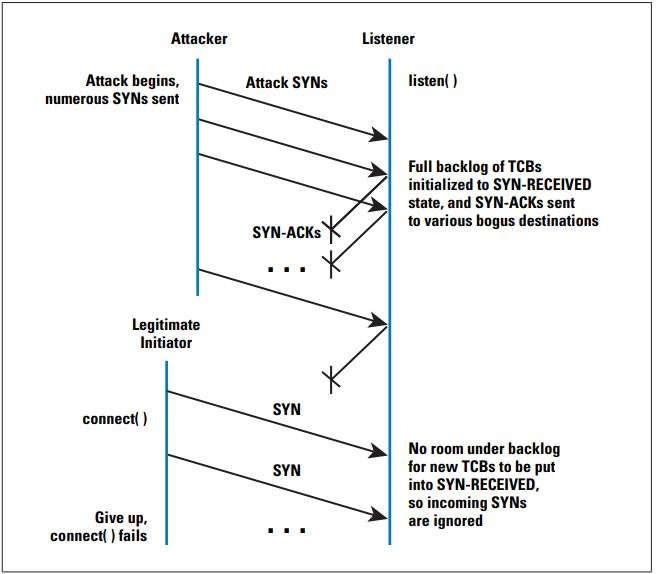
\includegraphics[scale=0.7]{SYNflood.jpg}
\caption{Voorbeeld van SYN-flood aaanval \autocite{eddy2006defenses} }
\label{fig:SYNflood}
\end{figure}  
 
\subsection{Neighbor Discovery}
In het IPv6-protocol is een ander kwetsbaar protocol het Neighbor Discovery (ND) protocol. Dit protocol wordt door apparaten binnen een netwerk gebruikt om informatie over de lokale topologie te verkrijgen, zoals IP- en MAC-adressen, evenals de IP-naar-MAC-mapping van aanwezige routers in het lokale netwerk. \autocite{nikander2004ipv6} Wat dit protocol risicovol maakt, is dat elk apparaat in het netwerk zichzelf kan presenteren als een router. \autocite{ullrich2014ipv6} Hierdoor ontstaat een potentiële mogelijkheid voor een hacker om een routeraankondiging te vervalsen. Deze vervalsing van de routeraankondiging kan ernstige gevolgen hebben voor het netwerkverkeer en de beveiliging ervan. Het kan leiden tot verkeerde routerselectie, waarbij pakketten worden doorgestuurd naar een valse router in plaats van de legitieme router, wat kan resulteren in packet loss of zelfs het mogelijk maken van man-in-the-middle-aanvallen. Bovendien kan het manipuleren van de time to live (TTL) van de router de normale routering van pakketten verstoren en de communicatie binnen het netwerk verstoren.


\subsection{Mobiliteit}
Mobiliteitsondersteuning direct in het protocol zelf integreren was een van de voornaamste doelstellingen van IPv6, in tegenstelling tot IPv4, waarbij gebruik wordt gemaakt van extensies zoals Mobile IP die mogelijk niet naadloos samengaan met onderliggende mechanismen.\autocite{ELGOARANY200732} Op gelijke wijze worden aanvullende beveiligingsextensies zoals IPsec en HTTPS vereist om beveiligingsproblemen aan te pakken bij IPv4, terwijl IPv6 streeft naar directe integratie van beveiligingskenmerken in het protocol.\autocite{sotillo2006ipv6} Mobiliteit maakt gebruik van twee soorten adressen: een permanent adres en een mobiel adres. Het permanente adres is een typisch IPv6-adres, terwijl het mobiele adres een tijdelijk adres is dat wordt gebruikt in de IP-header. Het mobiele adres kan kwetsbaar zijn voor spoofing-aanvallen. Netwerkbeheerders moeten zich bewust zijn van de complexiteit van mobiliteit en speciale veiligheidsmaatregelen toepassen.




\section{\IfLanguageName{dutch}{Mitigatie van IPv6}{De weg naar IPv6?}}%
\label{sec:De weg naar IPv6?}

\subsection{Header manipulation}
\textcite{boek1} leggen in hun boek uit ongeoorloofde pogingen tot headermanipulatie kunnen beperkt worden door het afdwingen van beveiligde netwerkconfiguraties. Dit omvat het configureren van netwerkapparaten en routers met strikte toegangscontrolelijsten (ACL's) en correcte filterregels. Op deze manier wordt ervoor gezorgd dat alleen legitiem en verwacht verkeer toegestaan wordt in het netwerk. Het scannen van een volledig IPv6-segment blijft een aanzienlijke tijdsinspanning vereisen, ondanks het gebruik van 64 bits voor IPv6-adressen, wat resulteert in een veel grotere adresruimte dan IPv4. Aanvankelijk lijkt het een onmogelijke taak om elk individueel adres te scannen, gezien de 2\^64 mogelijke unieke adressen. Zelfs met geavanceerde scantechnieken en enorme rekenkracht kan het doorlopen van elk adres in een volledig IPv6-segment tot wel 580 miljard jaar duren. \autocite{boek1} Het gebruik van de langere adresruimte betekent dus niet automatisch dat IPv6 veilig is. Er kan nog steeds gescanned worden met extra methoden die het taak minder intersief maken. Zo kan het netwerk kan nog steeds het slachtoffer worden van een flooding attack.

\subsection{Multicast adressen} 

Het beveiligen van multicast is historisch gezien een uitdaging vanwege de aard ervan. Het multicast-model omvat een enkele bron die naar meerdere ontvangers stuurt, waardoor het moeilijk is om traditionele beveiligingsmaatregelen toe te passen. \autocite{6726061} Toch is het mogelijk om deze aanvallen in IPv6 te verminderen, stelt \textcite{deering2000ipv6} dat een ICMPv6-bericht niet gegenereerd mag worden als reactie op een pakket met een IPv6 \newline multicast-bestemmingsadres, een link-layer multicast-adres of een link-layer \newline broadcast-adres. Aan de andere kant kan de smurf-aanval, zelfs als nodes voldoen aan RFC 2463, gebruik maken van de gegenereerde foutberichten Parameter problem
\newline

ICMPv6 message als reactie op een pakket bestemd voor een multicast-groep \autocite{vyncke2009ipv6}, en kan het pakketten gebruiken die werden gebruikt in een multicast-videostream, omdat multicast-videostream pad maximum transmission unit (MTU) discovery vereist. \textcite{vyncke2009ipv6} stellen dat dit de deur opent naar een amplificatieaanval. Om dit probleem aan te pakken, adviseren ze ook om rate limiting toe te passen op die ICMP-berichten: deze berichten moeten zeldzaam zijn in elk netwerk, zodat een rate limit (10 berichten/seconde) het correcte gebruik van deze berichten (path MTU discovery) kan toestaan, terwijl de amplificatieaanval wordt geblokkeerd. \textcite{6726061} vat het uitstekend samen, het belangrijkste is het waarborgen van de veiligheid van multicast. Het is van essentieel belang voor het succesvol implementeren van groepscommunicatietoepassingen in IPv6. Het beveiligen tegen verkenning, DoS-aanvallen met versterking en het beschermen van het multicast-model zelf zijn cruciale aspecten om mogelijke risico's te verminderen.

\subsection{TCP}
Om te voorkomen dat SYN-Flooding aanvallen plaatsvinden, zijn er verschillende methoden ontwikkeld. \autocite{morbitzer2013tcp} Een van deze methoden zijn SYNCookies. Bij het creëren van een sequentienummer voor het TCP-segment met de SYN- en ACK-vlag maakt de server specifieke keuzes en berekent het sequentienummer op basis van een tijdteller, de Maximum Segment Size (MSS) gekozen door de server en een geheime functie. Dit sequentienummer wordt de SYN-Cookie genoemd.
Een andere methode voor bescherming tegen SYN-Flooding is een SYN-cache. In tegenstelling tot SYN-Cookies wordt informatie over de half-open verbinding nog steeds op de server opgeslagen, maar wordt de hoeveelheid geheugen die nodig is om de verbinding te onthouden geminimaliseerd. Dit wordt gedaan door een hash-waarde op te slaan met informatie over de bron- en bestemmingsadres en -poort en een willekeurig gekozen geheim in plaats van de originele waarden. 
Bovendien verklaart \textcite{morbitzer2013tcp} dat er nog veel meer defensieve technieken zijn zoals het filteren en het vergroten van de backlog queue.


\subsection{Neighbor Discovery}

Een mogelijke oplossing om de beveiliging van Neighbor Discovery-berichten te verbeteren, is de implementatie van Secure Neighbor Discovery (SEND). SEND introduceert nieuwe opties die dit mogelijk maken. \autocite{arkko2005secure} \textcite{7726976} bevestigen in hun paper dat SEND een krachtig mechanisme is om IPv6-link-local communicatie te beveiligen. Hoewel SEND wordt beschouwd als een veelbelovende oplossing om het ND-protocol te beschermen, is de implementatie ervan niet eenvoudig en dus uitdagend.
\newline

Er bestaat nog steeds de mogelijkheid om te spoofen in een IPv6-netwerk. \autocite{1333418} Neighbor Discovery zorgt ervoor dat spoofing alleen mogelijk is bij toestellen in hetzelfde netwerksegment. Dit geldt echter niet voor een 6to4 transitienetwerk. Omdat dit netwerk gebruikmaakt van protocol-encapsulatie, kunnen er andere problemen optreden, zoals adres-spoofing. Als dit het geval is, wordt er een gespoofd adres gebruikt om het interne netwerkpakket te maskeren. \autocite{1333418}

\subsection{Mobiliteit}


Het bewustzijn van de inherente complexiteit van mobiliteit in netwerken is van essentieel belang voor netwerkbeheerders, vooral in het geval van IPv6. Het beheer van de mobiliteit van apparaten en het waarborgen van hun veiligheid vormen cruciale verantwoordelijkheden voor deze beheerders. \textcite{aura2006designing} omschrijven dat mobiliteit uitdagingen met zich meebrengt op het gebied van netwerkbeveiliging, waarbij het behoud van de vertrouwelijkheid, integriteit en beschikbaarheid van gegevens tijdens de verplaatsing van apparaten tussen diverse netwerken en locaties centraal staat.
\newline

Om deze uitdagingen succesvol aan te pakken, dienen netwerkbeheerders speciale veiligheidsmaatregelen te implementeren. Dit omvat het toepassen van beveiligingsmechanismen zoals IPsec (Internet Protocol Security) om de vertrouwelijkheid en integriteit van gegevens te waarborgen gedurende de overdracht tussen mobiele apparaten en netwerken. Daarnaast is het van belang dat netwerkbeheerders zich richten op het effectieve beheer van gebruikersidentiteiten en de implementatie van authenticatieprotocollen, zodat uitsluitend geautoriseerde gebruikers toegang krijgen tot het netwerk.


\section{\IfLanguageName{dutch}{IPv6 Toolkit}{IPv6 Toolkit}}%
\textcite{gont2013security} verklaren dat de introductie van hun "SI6 Networks' IPv6 Toolkit", gebruikers momenteel een alternatieve mogelijkheid bieden om hun \newline IPv6-netwerken te beveiligen en problemen op te lossen, waardoor een eerdere afhankelijkheid van THC's IPv6-AttackSuite doorbroken wordt. Deze toolkit heeft tot doel een uitgebreide beveiligingsanalyse en probleemoplossing te bieden voor IPv6-netwerken en implementaties, waarbij speciale aandacht wordt besteed aan de ontwikkeling van schone, draagbare en veilige code. Daarnaast is er een aanzienlijke inspanning geleverd om gebruikers te voorzien van gedegen documentatie ter ondersteuning van hun IPv6-beveiligingsactiviteiten.
\newline

Een opmerkelijk kenmerk van SI6 Networks' IPv6 Toolkit is dat het vrij beschikbaar is als open source software, waardoor het toegankelijk is voor een breed scala aan gebruikers die geïnteresseerd zijn in IPv6-beveiliging, ongeacht hun financiële mogelijkheden. Dit biedt de gebruikers de gelegenheid om te profiteren van de opgedane expertise en het toegewijde werk op het gebied van IPv6-beveiliging door SI6 Networks.
\newline

De twee auteurs van de IPv6 Toolkit zijn Fernando Gont en Marc Heuse. 
Fernando Gont is een zeer ervaren beveiligingsonderzoeker en consultant bij SI6 Networks. Met zijn expertise heeft hij uitgebreide beveiligingsbeoordelingen uitgevoerd op verschillende communicatieprotocollen. Een opmerkelijk aspect van de carrière van Fernando Gont is zijn actieve deelname aan de IETF. Als betrokken lid van deze invloedrijke organisatie heeft hij zijn kennis en inzichten bijgedragen aan de ontwikkeling en standaardisatie van internetprotocollen. \autocite{gont2013security} Zijn werk binnen de IETF getuigt van zijn toewijding om de beveiliging en betrouwbaarheid van netwerkinfrastructuren te verbeteren. Door samen te werken met andere experts in het veld heeft Fernando Gont een belangrijke rol gespeeld bij het stimuleren van vooruitgang op het gebied van netwerkbeveiliging.
Marc Heuse is een bekende onafhankelijke security-onderzoeker en consultant. Een opmerkelijke prestatie van Marc Heuse is zijn rol als oprichter van The Hacker's Choice . Dit platform getuigt van zijn expertise en passie voor het verkennen en verbeteren van beveiligingsmaatregelen. Naast zijn bijdragen als onderzoeker en consultant wordt Marc Heuse ook erkend als auteur van talrijke publieke beveiligingstools. Deze tools, waaronder thc-ipv6, hydra, amap, THCScan, SuSEfirewall 1 + 2 en vele anderen. \autocite{gont2013security}
Door het  werk van de beide auteurs hebben ze  een toewijding aan het bevorderen van het vakgebied cybersecurity laten zien. Hun uitgebreide ervaring en diverse vaardigheden hebben hun gevestigd als een betrouwbaar figuren in de branche, en hun bijdragen blijven een aanzienlijke impact hebben op de ontwikkeling en verbetering van beveiligingsmaatregelen.



%%=============================================================================
%% Methodologie
%%=============================================================================

\chapter{\IfLanguageName{dutch}{Methodologie}{Methodology}}%
\label{ch:methodologie}

%% TODO: Hoe ben je te werk gegaan? Verdeel je onderzoek in grote fasen, en
%% licht in elke fase toe welke stappen je gevolgd hebt. Verantwoord waarom je
%% op deze manier te werk gegaan bent. Je moet kunnen aantonen dat je de best
%% mogelijke manier toegepast hebt om een antwoord te vinden op de
%% onderzoeksvraag.





Er zullen experimenten worden uitgevoerd om de effectiviteit van verschillende mitigatietechnieken te beoordelen. Hiervoor zal een laboratoriumnetwerkopstelling worden gebruikt waarin verschillende beveiligingskwetsbaarheden worden geïntroduceerd. Het doel is om de effectiviteit van de mitigatietechnieken te evalueren bij het voorkomen of beperken van deze kwetsbaarheden. Ook worden bestaande hulpprogramma's en best practices voor het beperken van \newline IPv6-beveiligingskwetsbaarheden geëvalueerd via deze experimenten.

Om deze experimenten uit te voeren, wordt een kleinschalige laboratoriumnetwerkopstelling gebruikt met een Pfsense router, een Ubuntu LTS computer en een Windows Server met een IIS webserver. Om de experimenten uit te voeren, worden tools gebruikt uit de IPv6ToolKit, die beschikbaar zijn op \newline https://github.com/fgont/ipv6toolkit. Deze toolkit bevat verschillende tools die kunnen worden gebruikt voor het beoordelen van IPv6-beveiligingskwetsbaarheden en andere doeleinden. In dit onderzoek worden de volgende tools gebruikt:

\begin{itemize}
    \item	addr6: een IPv6 address analyse en manipulatie tool.
    \item	icmp6: een tool om aanvallen gebaseerd op ICMPv6 error berichten uit te voeren.
    \item	na6: een tool om kwaadwillige  Neighbor Advertisement berichten te verzenden.
    \item	ns6: een tool om kwaadwillige Neighbor Solicitation berichten te verzenden.
    \item	rs6: een tool om kwaadwillige Router Solicitation berichten te verzenden.
    \item	scan6: een IPv6 address scanning tool.
    \item	tcp6: een tool om kwaadwillige TCP segments uit te sturen en verschillende TCP-based attacks los te laten.
\end{itemize}

De tool wordt systematisch in het netwerk losgelaten, waarbij elk onderdeel van de tool wordt gebruikt om het netwerk te scannen en aan te vallen. Vervolgens wordt geanalyseerd hoe deze activiteiten werken en wat de impact is op het netwerk, met aandacht voor de omvang van de schade. Hierbij wordt gekeken naar de downtime van het netwerk en hoe snel het probleem kan worden opgelost.
Daarna worden alle bekende mitigatietechnieken toegepast in het netwerk en wordt de tool opnieuw gebruikt om de impact te vergelijken. Hierbij wordt gekeken naar het verschil in effectiviteit van de aanval na het toepassen van deze technieken. Zo kan worden vastgesteld of de aanval daadwerkelijk wordt vertraagd of volledig wordt voorkomen.

\section{Voorbereiding}
\subsection{laboratoriumnetwerkopstelling}
Als allereerste moet het de laboratoriumnetwerkopstelling opgesteld worden.. Het testlab zal een virtuele LAN zijn die  bestaan uit een virtuele router en virtuele machines (VM’s). De virtuele LAN zorgt ervoor dat het testlab geïsoleerd is van je fysieke LAN. Zo kunnen er veilige testen uitgevoerd worden. Het testlab zal volledig daaien in een virtualbox omgeving. VirtualBox is een gratis en open-source virtualisatiesoftware waarmee gebruikers virtuele machines kunnen maken en uitvoeren op hun computer. Je kan deze gemakkelijk installeren via \newline https://www.virtualbox.org/wiki/Downloads. 

\subsection{Pfsense router}
Om te beginnen wordt er een Pfsense router als virtuele machine geïnstalleerd in VirtualBox. Pfsense is een veelgebruikte open source firewall- en routeringssoftware die op een speciale computer of virtuele machine kan worden geïnstalleerd om te fungeren als router, firewall of ander netwerkbeveiligingsapparaat. Het is gebaseerd op het FreeBSD-besturingssysteem en wordt beheerd via een webgebaseerde grafische interface, waarmee netwerkinstellingen en -configuraties kunnen worden beheerd. Met pfSense kunnen verschillende netwerkfuncties worden gerealiseerd, zoals netwerkroutering, NAT en firewallfunctionaliteit.
De Pfsense router zal fungeren als firewall, DHCP en DNS server. Indien er een aparte internetverbinding beschikbaar is, kan er een aparte fysieke netwerkkaart worden toegewezen aan de computer om het virtuele LAN te voorzien van een publiek IP-adres. Het wordt echter verondersteld dat de meeste computers hier niet over beschikken en daarom zal deze stap worden overgeslagen.
De iso file die gebruikt wordt kan gedownload worden van volgende website: https://www.pfsense.org/download/.  Kies voor volgende attributen op de website. File Type: Install, Architecture: AMD64 (or whatever), Platform: CD Image (ISO Installer), voor de mirror kan je een plaats kiezen dicht in jouw buurt. Hier werd geopteerd voor Frankfurt, Duitsland. 

In virtualbox kies je voor volgende settings:
\begin{itemize}
    \item Memory size: 512MB 
    \item Create a virtual hard disk now
    \item Hard disk file type : VDI
    \item Storage on physical hard disk: dynamically allocated
    \item Onder storage word de gedownloade ISO tgeogevoegd als virtual optical Disk file
    \item Onder Network zorg je voor volgende instellingen
        \begin{itemize}
            \item Adapter 1
            \begin{itemize}
                \item Enable network adapter : on
                \item Attachted to: NAT
                
            \end{itemize}
        \end{itemize}
        \begin{itemize}
            \item Adapter 2
            \begin{itemize}
                \item Enable network adapter : on
                \item Attachted to: Internal Network (hier is het ‘testlab’)
                
            \end{itemize}
        \end{itemize}
    
\end{itemize}
Zodra de virtuele machine is opgezet, kan deze worden opgestart. Tijdens de installatie worden alle standaardinstellingen behouden. Zodra de installatie is voltooid, kan het ISO-optische bestand worden verwijderd en kan de virtuele machine opnieuw worden opgestart.
\newline

Na een succesvolle installatie kan de netwerkinterface worden toegewezen. Ga hiervoor naar optie 2 (Set interfaces IP address) in het PFsense menu. Met behulp van Autodetect worden de WAN- en LAN-interfaces automatisch toegewezen. Voor de LAN-interface wordt een statisch IP-adres toegewezen, bijvoorbeeld: 2001:db8:acad:10::1/64. Vervolgens wordt gevraagd om een DHCP-client in te stellen met een IPv6-adresreeks van 2001:db8:acad:10::1/64 tot 2001:db8:acad:10::9/64.
\newline

\subsection{LAN client}
Als tweede wordt er in het netwerk een LAN client geïnstalleerd. Deze zal een Ubuntu 14.04 LTS zijn. Ubuntu 14.04 LTS is een versie van het \newline Ubuntu-besturingssysteem met een focus op stabiliteit en ondersteuning op de lange termijn. Het is gebaseerd op de Linux-kernel en wordt ondersteund tot april 2019. 
\newline

De Unity-desktopomgeving biedt een moderne en gebruiksvriendelijke interface, samen met populaire toepassingen zoals Firefox, LibreOffice en \newline de GIMP-afbeeldingseditor. Ubuntu 14.04 LTS is ook ontworpen om gemakkelijk te gebruiken te zijn voor zowel nieuwe als ervaren gebruikers, met veel functies en tools. De ISO kan gedownload worden \footnote{https://www.releases.ubuntu.com/14.04/} . Er wordt een nieuwe virtual machine aangemaakt.
In virtualbox kies je voor volgende settings:
\begin{itemize}
    \item Memory size: 3072MB 
    \item Create a virtual hard disk now
    \item Hard disk file type : VDI
    \item Storage on physical hard disk: dynamically allocated
    \item Onder storage word de gedownloade ISO tgeogevoegd als virtual optical Disk file
    \item Onder Network zorg je voor volgende instellingen
    \begin{itemize}
        \item Adapter 1
        \begin{itemize}
            \item Enable network adapter : on
            \item Attachted to: Internal Network (hier is het ‘testlab’)
            
        \end{itemize}
    \end{itemize}
    
    
\end{itemize}

\subsection{Windows Server}
Als derde wordt er een windows server 2019 geïnstalleerd in het netwerk. De ISO \footnote{https://www.microsoft.com/en-us/evalcenter/download-windows-server-2019} kan gedownload worden.
In virtualbox kies je voor volgende settings:
\begin{itemize}
    \item Memory size: 2048MB 
    \item Create a virtual hard disk now
    \item Hard disk file type : VDI
    \item Storage on physical hard disk: dynamically allocated
    \item Onder storage word de gedownloade ISO tgeogevoegd als virtual optical Disk file
    \item Onder Network zorg je voor volgende instellingen
    \begin{itemize}
        \item Adapter 1
        \begin{itemize}
            \item Enable network adapter : on
            \item Attachted to: Internal Network (hier is het ‘testlab’)
            
        \end{itemize}
    \end{itemize}
    
    
\end{itemize}

\section{Configuratie}
Na een succesvolle installatie hebben zowel de Ubuntu als de Windows Server een IPv6-adres gekregen binnen de DHCP-range. Het IPv6-adres van Ubuntu is \newline 2001:db8:acad:10::9 en het IPv6-adres van de Windows Server is 2001:db8:acad:10::8.

\subsection{Pfsense}
Via de Ubuntu in hetzelfde netwerk als de Pfsense router kan de webconfigurator worden bereikt via de URL https://[ 2001:db8:acad:10::1]. Wanneer de webinterface van PfSense wordt geopend, zal elke browser de gebruiker waarschuwen voor een beveiligingsprobleem vanwege het gebruik van een zelfondertekend certificaat. Dit is echter normaal en kan gewoon worden genegeerd. Als de gebruiker Firefox of een afgeleide daarvan gebruikt, kan er op "Geavanceerd" worden geklikt, vervolgens op "Uitzondering toevoegen" en "Beveiligingsuitzondering bevestigen". Er kan worden ingelogd met de gebruikersnaam "admin" en het wachtwoord "pfsense". Om de virtuele LAN verder te isoleren van het fysieke LAN, kan er een firewallregel worden toegevoegd die verkeer van LAN naar het WAN-netwerk blokkeert, met uitzondering van de internetgateway. Maak onder firwall > rules een nieuwe regel aan met volgende eigenschappen.

\begin{itemize}
    \item  Actie: Blokkeren Interface
    \item LAN Adresfamilie: IPv4+IPv6 
    \item Protocol: Elke 
    \item Bron: LAN net 
    \item Bestemming: WAN net 
    \item Beschrijving: verkeer naar extern WAN niet toestaan 
    
\end{itemize}

\begin{figure}[H]
    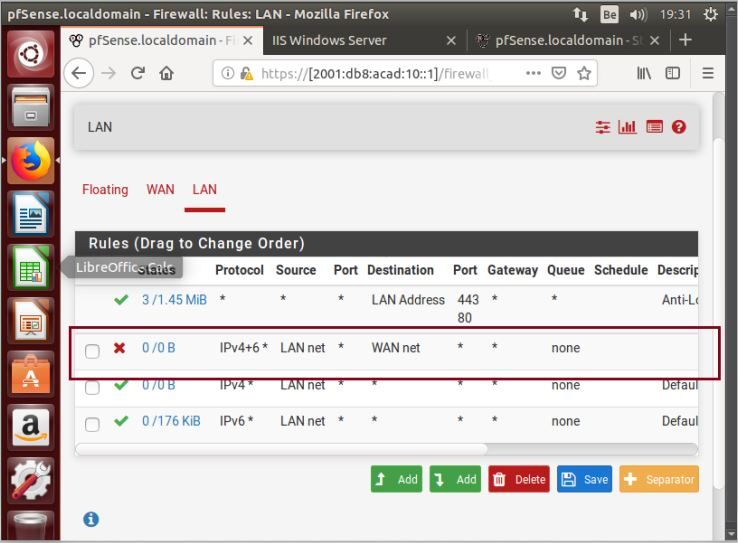
\includegraphics[scale=0.7]{Firewallrule.JPG}
    \caption{
        Een visuele weergave van de firewallregel. }
\end{figure}  

\subsection{Windows Server}

Op de Windows-server wordt een IIS-webserver geïnstalleerd om gemakkelijk te kunnen controleren wanneer de server niet meer beschikbaar is als gevolg van een aanval. Deze installatie kan eenvoudig worden uitgevoerd via de PowerShell-command line interface (CLI). 

\begin{lstlisting}[language=PowerShell,style=PowerShellStyle]
    Install-WindowsFeature -name Web-Server -IncludeManagementTools
\end{lstlisting}

\section{Uitvoering}
De volgende stap is het uitvoeren van de aanvallen vanuit de Ubuntu. Dit wordt gedaan met de IPv6Toolkit die te vinden valt op deze github \footnote{https://github.com/fgont/ipv6toolkit}: \newline . 
Je kunt de tools bouwen door het volgende commando uit te voeren:


\begin{lstlisting}[style=customStyleBashDark]
    make all
\end{lstlisting}
Je kunt de tools, het configuratiebestand, de database en bestaande handleidingen installeren door de volgende opdracht uit te voeren:

\begin{lstlisting}[style=customStyleBashDark]
    make install
\end{lstlisting}

Let op: de libpcap-bibliotheek moet al zijn geïnstalleerd op het systeem. Het overeenkomstige pakket heeft meestal de naam "libpcap-dev".

\subsection{Scanning }
Het scannen van het network kan gedaan worden met de Scan6 tool uit de IPv6toolkit. Er worden enkele scans uitgevoerd.
Er wordt hostscanning uitgevoerd op het lokale netwerk via de interface "eth0". Hierbij worden zowel ICMPv6-echoverzoeken gebruikt. De link-local adressen worden afgedrukt samen met de IPv6-adressen.

\begin{lstlisting}[language=PowerShell,style=PowerShellStyle]
    sudo scan6 \\-i eth0 \\-L \\-e \\-v
\end{lstlisting}
\begin{figure}[H]
    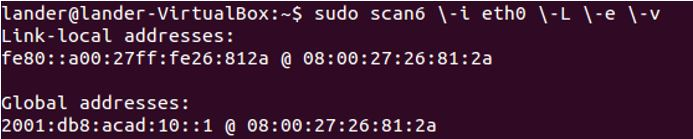
\includegraphics[scale=0.7]{Scan61.JPG}
    \caption{
       Output Scan6 op het lokaal netwerk }
       \label{fig:Scan61}
\end{figure}  

Bovendien wordt er nog een hostscanning uitgevoerd op het lokale netwerk via de "eth0" interface. Alleen globale unicast-adressen worden afgedrukt en er wordt maximaal één IPv6-adres per Ethernet-adres weergegeven. Ethernet-adressen worden samen met het bijbehorende IPv6-adres geprint.
\begin{lstlisting}[language=PowerShell,style=PowerShellStyle]
    scan6 \-i eth0 \-L \-P global \-\-print\-unique \-e
\end{lstlisting}
\begin{figure}[H]
    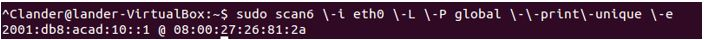
\includegraphics[scale=0.7]{Scan62.JPG}
    \caption{
        Output tweede Scan6 op het lokaal netwerk }
        \label{fig:Scan62}
\end{figure}  

\subsection{Header analyzing/manipulation }

Met de Addr6 tool kan er IPv6 adrressen  geanalyseerd worden. 


Eerst en vooral wordt de statistiek van het IPv6-adres geanalyseerd. Dit gaat met het volgende commando:

\begin{lstlisting}[language=PowerShell,style=PowerShellStyle]
    echo "2001:db8:acad:10::8" | addr6 -i -s
\end{lstlisting}
Als er meerdere IPv6-adressen geanalyseerd moeten worden, bestaat de mogelijkheid om een lijst van IPv6-adressen in te voeren in het commando. Dit ziet er dan als volgt uit:
\begin{lstlisting}[language=PowerShell,style=PowerShellStyle]
    cat MyListIPv6.txt | addr6 -i -s
\end{lstlisting}

\begin{figure}[H]
    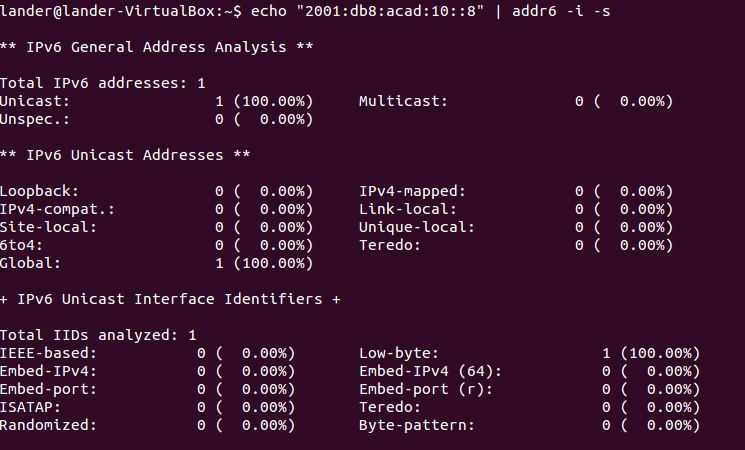
\includegraphics[scale=0.7]{StatisAddress.JPG}
    \caption{
        Output Addr6 analyze statistiek }
        \label{fig:StatisAddress}
\end{figure} 



Bij het gebruik van de Addr6 tool kunnen lijsten met IPv6-adressen gegenereerd worden. Echter, niet alle adressen in de lijst zijn mogelijk relevant of nuttig. In dergelijke gevallen kan het handig zijn om verschillende filters toe te passen om de groep IPv6-adressen te verfijnen. Deze filters kunnen onder andere het verwijderen van dubbele adressen uit de lijst, het elimineren van adressen die niet behoren tot een specifiek voorvoegsel, of het verkrijgen van adressen van een specifiek bereik omvatten. Door gebruik te maken van deze filtertechnieken wordt de resulterende lijst van IPv6-adressen meer gericht en afgestemd op de specifieke vereisten van het beoordelingsproces.

De voorbeelden worden even opgesomd: 

\begin{itemize}
    \item  Verwijder dubbele adressen:
    \begin{lstlisting}[language=PowerShell,style=PowerShellStyle]
        addr6 -i -q
    \end{lstlisting}
    \item Accepteer of blokeer specifieke prefix: 
    \begin{lstlisting}[language=PowerShell,style=PowerShellStyle]
        addr6 --accept PREFIX
    \end{lstlisting}
    \item Accepteer of blokeer adres types:
    \begin{lstlisting}[language=PowerShell,style=PowerShellStyle]
        addr6 --accept-type TYPE
    \end{lstlisting}
  \item Accepteer of blokeer adres scopes:
  \begin{lstlisting}[language=PowerShell,style=PowerShellStyle]
      addr6 --accept-scope SCOPE
        \end{lstlisting}
    \item Accepteer of blokeer unicast adres typen:
  \begin{lstlisting}[language=PowerShell,style=PowerShellStyle]
      addr6 --accept-utype TYPE
      \end{lstlisting}
\end{itemize}


\subsection{Multicast Adressen}
Met behulp van het volgende commando kan een aanval worden uitgevoerd met behulp van ICMPv6-foutpakketten:
\begin{lstlisting}[language=PowerShell,style=PowerShellStyle]
    icmp6 \-\-icmp6\-packet\-too\-big \-p ICMP6 \-d 2001:db8:acad:10::1 \-\-peer\-addr 2001:db8:acad:10::8 \-m 1240 \-v 
\end{lstlisting}

De tool genereert een ICMPv6-foutbericht van het type "Packet Too Big". Dit foutbericht adverteert een Maximum Transmission Unit (MTU) van 1240 bytes. Het wordt verzonden naar het adres "2001:db8:acad:10::1". Binnen dit ICMPv6-foutbericht wordt een ICMPv6 Echo Request-bericht opgenomen. Het bronadres van dit Echo Request-bericht is ingesteld op "2001:db8:10::1", wat hetzelfde adres is als het bestemmingsadres van het foutbericht. Het bestemmingsadres is ingesteld op \newline "2001:db8:acad:10::8". De waarden van de velden "Identifier" en "Sequence Number" van het ingebedde ICMPv6 Echo Request-bericht worden willekeurig gegenereerd. Bovendien wordt alle informatie weergegeven door het aanroepen van de verbose optie.

\begin{figure}[H]
    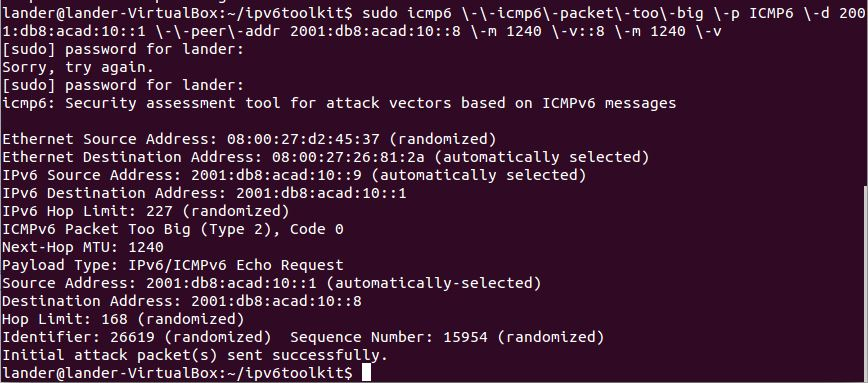
\includegraphics[scale=0.7]{ICMPcmd.JPG}
    \caption{
        Output voor de ICMPv6-aanval }
        \label{fig:ICMPcmd}
\end{figure}  

Op dit moment is het helaas nog niet mogelijk om met de huidige tool ICMPv6-content te controleren, wat betekent dat te grote pakketten nog steeds kunnen doorgaan. Deze functionaliteit is een toevoeging die nog moet worden geïmplementeerd in de IPv6-ToolKit. Gelukkig is het wel mogelijk om deze aanval te beperken door het instellen van een firewall. Door een firewall in te stellen, kunnen ongewenste pakketten worden tegengehouden en kan de netwerkbeveiliging worden versterkt.
In PFsense wordt een firewallregel ingesteld om verkeer van ICMPv6 "Packet too big" te filteren op basis van het bestemmingsadres. Vervolgens wordt de aanval opnieuw uitgevoerd. Op de figuur \ref{fig:ICMPv6} hieronder wordt de firewallregel weergegeven.

\begin{figure}[H]
    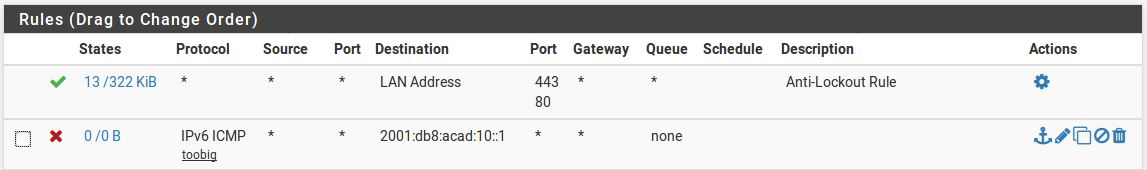
\includegraphics[scale=0.7]{FirewallTooBig.JPG}
    \caption{
        Weergave van de ICMPv6 firewallregel }
        \label{fig:ICMPv6}
\end{figure}  


\subsection{TCP}
Voordat de aanval op TCP uitgevoerd wordt, wordt er gecontroleerd of deze poort daadwerkelijk actief is met behulp van Nmap. Het volgende commando bereikt dit: 
\begin{lstlisting}[language=PowerShell,style=PowerShellStyle]
     nmap -6 -p 80 2001:db8:acad:10::8 
\end{lstlisting}
 Op de onderstaande foto zie je de uitvoer en het bewijs dat de poort inderdaad actief is.
 \begin{figure}[H]
     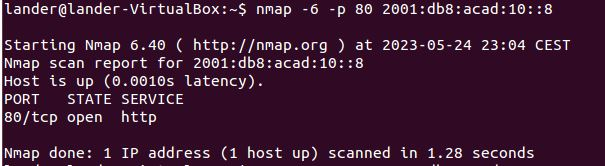
\includegraphics[scale=0.6]{NmapUP.JPG}
     \caption{
         Output voor de Nmap port 80 }
         \label{fig:Nmap1}
 \end{figure}  
 
 Vervolgens wordt de TCP-SYN-aanval uitgevoerd met het volgende commando:
\begin{lstlisting}[language=PowerShell,style=PowerShellStyle]
     sudo tcp6 -s 2001:db8:acad:10::/64 -d 2001:db8:acad:10::8 -a 80 -X S -F 100000 -l -z 1 -v
\end{lstlisting}
 \begin{figure}[H]
    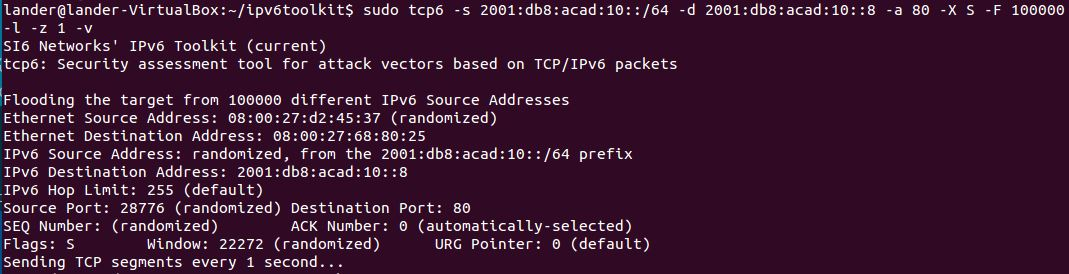
\includegraphics[scale=0.7]{TCPattack.JPG}
    \caption{
        Output van de TCP-aanval }
        \label{fig:TCPattack}
\end{figure}  

Deze tool lanceert een SYN-flood aanval op poortnummer 22 van de host \newline 2001:db8:acad:10::8. Het maakt gebruik van het netwerkinterface "eth0" en stuurt SYN-segmenten vanaf het prefix 2001:db8:acad:10::/64 naar poort 80 op het doeladres 2001:db8:acad:10::8. De tool verzendt TCP-segmenten vanaf 100.000 verschillende adressen met een interval van één seconde. Bovendien wordt de verbose optie gebruikt, zodat de tool gedetailleerde informatie zal tonen.

Tijdens de aanval kan opnieuw een Nmap-scan worden uitgevoerd, waarbij wordt aangegeven dat de poort als inactief wordt beschouwd. Dit bevestigt het succes van de aanval.

 \begin{figure}[H]
    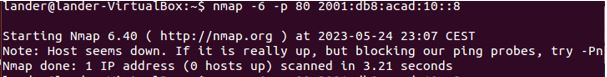
\includegraphics[scale=0.7]{NmapDOWN.JPG}
    \caption{
        Output voor de Nmap port 80 tijdens de aanval }
        \label{fig:Nmap2}
\end{figure}  

Als de aanval wordt uitgevoerd op een Ubuntu-systeem, kunnen SYN-cookies gemakkelijk worden ingesteld. Dit kan worden gedaan door het bestand sysctl.conf te openen met het volgende commando.

\begin{lstlisting}[language=PowerShell,style=PowerShellStyle]
    sudo nano /etc/sysctl.conf
\end{lstlisting}
Vervolgens worden de volgende vier regels aan het bestand toegevoegd en wordt het opgeslagen.
\begin{itemize}
     
    \item  net.ipv4.tcp\_syncookies = 1
    \item  net.ipv4.tcp\_synack\_retries = 3
    \item  net.ipv4.tcp\_max\_syn\_backlog = 2048
    \item  net.ipv4.tcp\_syncookie\_max\_age = 120
    
\end{itemize}


Het instellen van "tcp\_synack\_retries" zorgt ervoor dat er slechts drie \newline SYN/ACK-herkansingen plaatsvinden voordat een verbinding wordt opgegeven. \newline "tcp\_max\_syn\_backlog" stelt de maximale wachtrijgrootte in op 2048 verzoeken voor het ontvangen van nieuwe SYN-verzoeken. "tcp\_syncookie\_max\_age" stelt de maximale levensduur van een SYN-cookie in op 120 seconden.

Herlaad de systeemconfiguratie met de nieuwe wijzigingen:
\begin{lstlisting}[language=PowerShell,style=PowerShellStyle]
    sudo sysctl -p
\end{lstlisting}

In Windows Server is er geen specifieke configuratieoptie voor SYN-cookies, zoals beschikbaar in Linux-gebaseerde systemen. SYN-cookies zijn een mechanisme dat voornamelijk wordt gebruikt in Linux-kernels om SYN-floodingaanvallen tegen te gaan.
\newline

In Windows Server wordt de aanval echter aangepakt door firewallregels in te stellen. Dit wordt gedaan door de bronadressen van legitiem verkeer te identificeren. Dit verkeer wordt doorgelaten op poort 80, terwijl de andere IP-adressen worden geblokkeerd.

\subsection{Neighbor Discovery}

Met behulp van de ra6.1 tool kunnen diverse aanvallen worden uitgevoerd, waarbij in dit geval een flooding aanval wordt toegepast. Het commando dat wordt gebruikt om deze aanval uit te voeren, is als volgt:

\begin{lstlisting}[language=PowerShell,style=PowerShellStyle]
    sudo ra6 \-i eth0 \-s fe80::1234 \-S 08:00:27:d2:45:37 \-d FF02::1 \-N 900 \-\-flood\-dns 10#10 \-L
\end{lstlisting}

Bij deze aanval worden er 10 willekeurige IPv6-adressen van Recursive DNS-servers verzonden naar het doeladres FF02::1, waarbij elke RDNSS-optie maximaal 10 adressen bevat. Elke RDNSS-optie heeft een levensduur van 900. De pakketten worden verstuurd met een IPv6-bronadres van fe80::1234 en een Ethernet-bronadres van 00:01:02:03:04:05. Nadat het doelwit is aangevallen, wordt er geluisterd naar inkomende Router Solicitation-berichten en wordt er gereageerd met dezelfde "overstromings"pakketten.

Het bovenstaande commando demonstreert de manier waarop de ra6.1 tool wordt gebruikt om de flooding aanval uit te voeren, waarbij verschillende parameters worden ingesteld om de aanval te configureren en de gewenste effecten te bereiken.
\chapter{\IfLanguageName{dutch}{Resultaten}{Results}}%
\label{ch:resultaten}

Er wordt een grondige evaluatie gemaakt van de bevindingen. Hierbij wordt opgemerkt dat bij het onderzoeken van het netwerk de juiste resultaten worden verkregen. Bij het uitvoeren van de hostscanning wordt duidelijk waargenomen in figuur \ref{fig:Scan61} dat zowel een link-local adres als een global adres worden weergegeven. Het resultaat omvat dus zowel het link-local adres als het global adres. Bovendien bestaat er een scanmethode waarbij alleen de globale unicast-adressen op het scherm worden afgedrukt. Dit specifieke resultaat wordt getoond in figuur \ref{fig:Scan62}.


\newline

De Addr6-tool biedt een waardevol hulpmiddel om gedetailleerde statistieken van het IPv6-adres 2001:db8:acad:10::8 te bekijken. In figuur \ref{fig:StatisAddress} wordt een overzichtelijke weergave van deze statistieken gepresenteerd, waardoor een dieper inzicht ontstaat in de eigenschappen en kenmerken van het betreffende adres. Deze tool gaat verder dan alleen het verstrekken van statistieken en biedt ook de mogelijkheid om filterregels in te stellen.
\newline

Door gebruik te maken van de Addr6-tool kunnen filterregels worden geconfigureerd, waardoor het mogelijk is om alleen specifieke adressoorten te accepteren op het adres 2001:db8:acad:10::8. Dit betekent dat het netwerkbeheerders in staat stelt om nauwkeurige controle uit te oefenen over welke soorten verkeer worden toegestaan op dit specifieke IPv6-adres. Bovendien kunnen dezelfde principes worden toegepast op bepaalde adres scopes, waardoor een meer geavanceerd beheer van het IPv6-netwerk mogelijk wordt.

\newline

De uitgevoerde aanval met behulp van ICMPv6-foutpakketten heeft zich bewezen als een succesvolle poging. Met de specifieke tool was het mogelijk om een "Packet too big" bericht te sturen naar de Pfsense-router. Als reactie op dit bericht verzond de Pfsense-router een ICMPv6 Echo Request-bericht naar het opgegeven doeladres, namelijk het IP-adres van de Windows-server. Na exact 15 seconden werd het duidelijk dat de webserver, die op de Windows-server draait, niet langer toegankelijk was. De aanval bleek dus succesvol te zijn en de webserver herstelde niet automatisch zijn online functionaliteit. Om de webserver weer operationeel te maken, was het noodzakelijk om de Windows-server opnieuw op te starten.
\newline

Na het realiseren van de potentiële kwetsbaarheid van de webserver als gevolg van de succesvolle aanval, werd er besloten om een versterkte beveiligingsmaatregel te implementeren. In dit geval werd een firewallregel toegevoegd aan de Pfsense-router, met als doel het filteren van ICMPv6-foutberichten. Nadat deze firewallregel was toegepast, werd de aanval opnieuw uitgevoerd om te testen of de webserver nu weerstand kon bieden aan de eerdere aanval. Deze keer resulteerde de aanval echter niet in het uitvallen van de webserver en bleef deze succesvol functioneren.
\newline

De succesvolle werking van de webserver, zelfs na herhaalde pogingen tot aanval, wijst onmiskenbaar op de doeltreffendheid van de toegepaste firewallregel op de Pfsense-router. Het bewijs van de firewall's vermogen om ICMPv6-foutberichten te filteren en daarmee de aanvallen af te weren, toont aan dat de genomen maatregelen effectief zijn bij het versterken van de beveiliging van het netwerk.
\bigskip
\newline

Bij het uitvoeren van de TCP-SYN-aanval werden interessante bevindingen waargenomen. Het viel op dat poort 80 van de Windows-server (2001:db8:acad:10::8) open was en toegankelijk was zoals geïllustreerd in figuur \ref{fig:Nmap1}. Vervolgens slaagde de aanval erin om de doelpoort te overstromen met maar liefst 10.000 verschillende IPv6-bronadressen. Wat deze aanval nog uitdagender maakte, was dat de gebruikte tool in staat was om de bronpoort en SEQ-nummers willekeurig te genereren, waardoor de complexiteit van het tegengaan van deze aanval toenam. Na de aanval bevestigde een Nmap-scan, te zien op figuur \ref{fig:Nmap2}, van poort 80 dat deze niet langer actief was en niet meer kon worden gebruikt.
\newline

Interessant genoeg blijkt dat als de aanval gericht is op een Ubuntu-systeem, deze kan worden afgeweerd door het toevoegen van een SYN-cookie. Nadat de systeemconfiguratie opnieuw was geladen, werd het Ubuntu-systeem opnieuw aangevallen en werd de aanval succesvol geblokkeerd. In het geval van de Windows-server ligt de situatie echter anders. Daar moet de aanval worden tegengehouden door middel van een specifieke firewallregel. Dit benadrukt de noodzaak van verschillende beveiligingsmaatregelen, afhankelijk van het specifieke besturingssysteem, om effectieve bescherming te bieden tegen TCP-SYN-aanvallen.
\newline

Door de uitvoering van de flooding attack gebaseerd op router advertisements, resulteerde dit in een volledige uitval van het netwerk. De servers moesten opnieuw opgestart worden. Zelfs na de herstart was er nog steeds geen nieuw netwerkverkeer. Om het netwerk weer operationeel te krijgen, moeten de servers teruggezet worden naar hun oude snapshots, zodat alles weer in de vorige staat is hersteld. Dit impliceert dat de aanval een aanzienlijke impact heeft gehad op het netwerk, aangezien het zelfs na een herstart niet kon worden opgelost. Het is mogelijk dat een fout in de uitvoering van de aanval ook heeft bijgedragen aan de netwerkuitval met deze omvang. Hoe dan ook, is het van cruciaal belang om inkomend verkeer te filteren. Op die manier kunnen firewall-regels of netwerkapparatuur worden gebruikt om inkomend verkeer van onbekende of verdachte bronnen te blokkeren. Hierdoor kunnen de "flood" pakketten worden gestopt voordat ze het beoogde doel bereiken.


% Voeg hier je eigen hoofdstukken toe die de ``corpus'' van je bachelorproef
% vormen. De structuur en titels hangen af van je eigen onderzoek. Je kan bv.
% elke fase in je onderzoek in een apart hoofdstuk bespreken.

%\input{...}
%\input{...}
%...

%%=============================================================================
%% Conclusie
%%=============================================================================

\chapter{Conclusie}%
\label{ch:conclusie}

% TODO: Trek een duidelijke conclusie, in de vorm van een antwoord op de
% onderzoeksvra(a)g(en). Wat was jouw bijdrage aan het onderzoeksdomein en
% hoe biedt dit meerwaarde aan het vakgebied/doelgroep? 
% Reflecteer kritisch over het resultaat. In Engelse teksten wordt deze sectie
% ``Discussion'' genoemd. Had je deze uitkomst verwacht? Zijn er zaken die nog
% niet duidelijk zijn?
% Heeft het onderzoek geleid tot nieuwe vragen die uitnodigen tot verder 
%onderzoek?



Het scannen van IPv6-adressen biedt een waardevol perspectief op de structuur van een netwerk en helpt bij het ontdekken van potentiële kwetsbaarheden. Door systematisch de IPv6-adressen binnen een netwerk te scannen en te analyseren, kan een beter inzicht worden verkregen in de lay-out en configuratie van het netwerk. Dit stelt netwerkbeheerders in staat om een gedetailleerd overzicht te krijgen van de verbonden apparaten, subnetten en de algehele topologie van het IPv6-netwerk.
Het scannen van IPv6-adressen biedt ook een belangrijk middel om kwetsbaarheden en beveiligingsrisico's te ontdekken. Door het uitvoeren van gerichte scans kunnen potentiële zwakke punten en blootstellingen in het netwerk worden geïdentificeerd. Dit omvat bijvoorbeeld het detecteren van open poorten, ongepatchte systemen, onveilige configuraties en andere potentiële beveiligingslekken. Het verkrijgen van dit inzicht stelt netwerkbeheerders in staat om proactief maatregelen te nemen om de beveiliging te verbeteren, kwetsbaarheden te patchen en risico's te minimaliseren.
\newline

Deze functionaliteit van de Addr6-tool biedt aanzienlijke voordelen voor het beheer en de configuratie van het IPv6-netwerk. Door gerichte filterregels in te stellen, kunnen netwerkbeheerders ervoor zorgen dat alleen het gewenste verkeer wordt toegelaten op het adres 2001:db8:acad:10::8. Dit helpt bij het handhaven van een geoptimaliseerde en veilige netwerkomgeving, waarbij ongewenst verkeer en mogelijke bedreigingen worden geweerd. Bovendien vereenvoudigt de Addr6-tool het beheerproces door een intuïtieve en gebruiksvriendelijke interface te bieden, waardoor netwerkbeheerders efficiënter kunnen werken en snel de gewenste adresconfiguratie kunnen waarborgen.
Kortom, de Addr6-tool biedt waardevolle functionaliteit voor het beheer van IPv6-netwerken. Van het bekijken van gedetailleerde statistieken van specifieke IPv6-adressen tot het configureren van filterregels, deze tool draagt bij aan een geavanceerd en gestroomlijnd netwerkbeheerproces.
\newline

De aanval met ICMPv6 error-pakketten onderstreept opnieuw hoe eenvoudig het is om een dergelijke aanval uit te voeren en de mogelijke gevolgen die dit kan hebben voor een bedrijf. Het verontrustende feit is dat deze aanval kan worden uitgevoerd zonder uitgebreide voorkennis, aangezien online tools direct beschikbaar zijn voor kwaadwillende individuen. Deze aanval heeft het potentieel om aanzienlijke schade toe te brengen aan een organisatie, met name aan slecht geconfigureerde servers die gevoelig zijn voor dergelijke aanvallen.

Het zorgwekkende aspect van deze aanval is dat het mogelijk is om servers direct plat te leggen zonder enig voorafgaand waarschuwingssignaal van een aanval. Dit betekent dat een bedrijf zich mogelijk niet bewust is van de aanval totdat de servers onbereikbaar worden en de bedrijfsactiviteiten ernstig verstoord worden. Dit benadrukt het belang van proactieve maatregelen om de beveiliging van het netwerk te versterken en potentiële aanvallen voor te zijn.
\newline

Gelukkig kan de impact van ICMPv6 error-aanvallen aanzienlijk worden verminderd door het nemen van passende beveiligingsmaatregelen, met name door het configureren van firewalls. Door de kennis en expertise van de netwerkbeheerder te benutten, kunnen firewalls worden geconfigureerd om deze specifieke aanvallen te detecteren en te blokkeren. Hierdoor wordt de kwetsbaarheid van het netwerk verminderd en worden servers beter beschermd tegen potentieel schadelijke verkeersstromen.
\newline

Het is essentieel dat organisaties zich bewust zijn van de risico's van ICMPv6 error-aanvallen en zich inzetten voor een robuuste beveiligingsinfrastructuur. Dit omvat het regelmatig evalueren en verbeteren van de serverconfiguraties, het implementeren van firewalls en andere geavanceerde beveiligingsmaatregelen, en het investeren in de ontwikkeling van het beveiligingsbewustzijn van medewerkers.
Het is duidelijk dat het implementeren van passende beveiligingslagen van cruciaal belang is om de kwetsbaarheid van systemen te verminderen en de integriteit van het netwerk te waarborgen. De resultaten van deze aanval demonstreren het belang van proactieve beveiligingsmaatregelen, zoals SYN-cookies en firewallregels, om potentiële aanvallen te voorkomen of hun impact te minimaliseren. Door te erkennen dat verschillende besturingssystemen verschillende reacties vereisen op TCP-SYN-aanvallen, kunnen beveiligingsteams gerichte maatregelen nemen om de specifieke zwakke punten van elk systeem te versterken. Deze geïntegreerde aanpak draagt bij aan een veerkrachtige beveiligingsinfrastructuur die zich aanpast aan de evoluerende bedreigingslandschappen en zorgt voor een betrouwbaar en veilig netwerk.
\newline

Een belangrijke focus van het onderzoek is het gebruik van opensource tools voor mitigatie van IPv6-aanvallen. Opensource tools bieden vaak flexibiliteit, transparantie en een gemeenschapsgerichte benadering van beveiliging. Door het potentieel van opensource tools te benutten, kunnen beveiligingsexperts oplossingen ontwikkelen die zowel effectief als kostenefficiënt zijn voor kleinere bedrijven.

%---------- Bijlagen -----------------------------------------------------------

\appendix

\chapter{Onderzoeksvoorstel}

Het onderwerp van deze bachelorproef is gebaseerd op een onderzoeksvoorstel dat vooraf werd beoordeeld door de promotor. Dat voorstel is opgenomen in deze bijlage.

%% TODO: 
%\section*{Samenvatting}

% Kopieer en plak hier de samenvatting (abstract) van je onderzoeksvoorstel.

% Verwijzing naar het bestand met de inhoud van het onderzoeksvoorstel
%---------- Inleiding ---------------------------------------------------------

\section{Introductie}%
\label{sec:introductie}

Het Internet protocol (IP) is het meest gebruikte protocol. Dit zorgt er op zijn beurt voor dat de beveiliging ervan een topprioriteit is. De beveiliging gebeurt vooral door de Internet Engineering Task Force (IETF). Dit is de organisatie verantwoordelijk voor de IP-standaarden. Bij het uitrollen van IPv4 hadden ze niet geanticipeerd op de exponentiële groei van het internet. Dit zorgde ervoor dat nood was aan een opvolger van IPv4. Hieruit kwam IPv6. IPv6 was het natuurlijke gevolg van de evolutie van het internet. Hoewel de nood aan IPv6 groot was, gebruikt nog niet iedereen het protocol. De wereld bevindt zich nu in een transitie fase. De vraag is niet of iedereen IPv6 gaat gebruiken maar wanneer. Nieuwe protocollen brengen natuurlijk ook nieuwe kwetsbaarheden mee die vaak nog onbekend zijn bij IT’ers. Veel van IPv6-implementaties zijn nog niet in de praktijk getest.  Hierdoor heeft IPv6 wel de aandacht getrokken van mogelijke hackers. Daarom is het belangrijk dat bedrijven die overstappen naar een Ipv6-netwerk goed weten wat ze moeten doen voor ze dit implementeren. Daarom zullen in deze bachelorproef, volgende onderzoeksvragen onderzocht worden:
\begin{itemize}
  \item Wat zijn de veelvoorkomende beveiligingsproblemen in verband met IPv6?
	\item Wat zijn de hoofdoorzaken van deze kwetsbaarheden? 
 \item 	Wat is de impact van deze kwetsbaarheden op de netwerkbeveiliging?
\item	Welke mitigatietechnieken en aanbevolen procedures zijn beschikbaar om deze kwetsbaarheden te beperken?
 \item	Hoe effectief zijn deze mitigatietechnieken en -praktijken bij het beperken van {beveiligingskwetsbaarheden} van IPv6?
\end{itemize}

In deze bachelor proef wordt er voorgesteld om de veel voorkomende beveiligingskwetsbaarheden in verband met IPv6 te onderzoeken en de effectiviteit van verschillende mitigatietechnieken te evalueren. Het onderzoek zal zich richten op het identificeren van de onderliggende oorzaken van deze kwetsbaarheden en het onderzoeken van de impact die ze hebben op de netwerkbeveiliging. Er wordt ook de beschikbaarheid en effectiviteit van tools en best practices voor het beperken van deze kwetsbaarheden onderzocht worden. De bevindingen van het onderzoek zullen nuttig zijn voor netwerkbeheerders en beveiligingsprofessionals bij het verbeteren van de beveiliging van hun netwerken met behulp van IPv6.

%---------- Stand van zaken ---------------------------------------------------

\section{State-of-the-art}%
\label{sec:state-of-the-art}

Het implementeren van IPv6 blijft hoognodig. Hoewel NAT tijdelijk het probleem heeft opgelost voor het tekort aan IP-adressen is het niet adequaat. Deering verwijst hierbij naar onderstaande problemen \autocite{deering2000ipv6}:

\begin{itemize}
    \item	NAT zorgt voor problemen bij de meeste huidige IP-multicast- en IP-mobiliteit Protocollen 
    \item	NAT zorgt voor problemen bij veel bestaande applicaties  
    \item	NAT beperkt de markt voor nieuwe toepassingen en diensten
    \item	NAT brengt de prestaties, robuustheid, veiligheid en beheerbaarheid van het internet naar beneden
\end{itemize}
Men kan zich de vraag stellen “Waarom verbeteren we niet gewoon de gebreken van NAT?”. \textcite{deering2000ipv6} heeft een antwoord hiervoor. Hij schrijft dat dit alleen maar de complexiteit zal verhogen. Bovendien komen er extra gebreken bovenop. Het implementeren van IPv6 zal ervoor zorgen dat er nog veel andere veranderingen nodig zullen zijn tijdens de groei van het internet.

IP version 6 (IPv6) is de volgende generatie van het internetprotocol. Dit wil niet zeggen dat het een vervolg is op IPv4. Het is een volledig nieuw protocol. In tegenstelling tot het 32-bit adres van IPv4 is het IPv6 adres 128 bits lang. Hierdoor zijn er in theorie 3 biljoen adressen per persoon op de aarde. \textcite{andress2005ipv6} legt in zijn artikel uit dat de grote marge voor IP-adressen niet zo bedoeld is. Veel van de adresbits worden minder efficiënt gebruikt om het configureren van adressen te vergemakkelijken. Er zijn zeker nog genoeg adressen vrij voor gebruik in de toekomst \autocite{andress2005ipv6}. In de volgende sectie zal er besproken worden in welke gebieden de beveiliging van IPv6 beter kan.

Als je kijkt vanuit een beveiligingstandpunt is IPv6 een vooruitgang op het oude IPv4-protocol. Ondanks alle verbeteringen blijft IPv6 ver van veilig \autocite{sotillo2006ipv6}.
\textcite{sotillo2006ipv6} kaart in zijn paper het gevaar aan van header manipulation. De implementatie van extension headers en IPsec zorgen ervoor dat de vele header manipulation aanvallen worden tegengehouden. Het feit dat alle extension headers door alle stacks moeten verwerkt worden, kan zorgen voor problemen. Een lange keten van extension headers kan gebruikt worden om bepaalde knooppunten te overweldigen of het maskeren van een aanval. \textcite{boek1} legt in zijn boek uit dat de aanbevolen procedures aanraden het verkeer te filteren met niet ondersteunende diensten. 

Door het gebruik van 64 bits kan het scannen van een volledig IPv6 segment tot 580 miljard jaar duren \autocite{boek1}. Het gebruik van de langere adres ruimte wil dus niet zeggen dat IPv6 veilig is. Zo kan het netwerk nog altijd slachtoffer zijn van een flooding attack. 

Nieuwe features als multicast adressen zorgen voor problemen \autocite{1619968}. Nieuwe types ICMPv6-berichten en afhankelijkheid van multicast-adressen in IPv6 kan nieuwe manieren van misbruik bij flooding attacks bieden. ICMPv6-berichten moeten altijd toegelaten worden in een netwerk omdat ze nodig zijn voor een werkend netwerk \autocite{DURDAGI20105285}. Dit zorgt ervoor dat er ook error notificatie berichten kunnen verzonden worden naar multicast-adressen in het netwerk. Die kunnen misbruikt worden door hackers. Hackers zenden dan een gepast pakket naar een multicast-adres zodat ze meerdere berichten gericht op een slachtoffer kunnen sturen.
Een flooding attack kan ook plaatsvinden via het transmission control protocol (TCP) \autocite{gao2014detecting}. Deze aanval maakt gebruik van het  three way handshake mechanisme van het protocol. \textcite{gao2014detecting} leggen in hun paper uit hoe zo een aanval tot stand komt. Het aanvallend toestel kan een reeks SYN-verzoeken met een vervalst scource adres sturen naar een slachtoffer. Het slachtoffer stuurt dan een SYN/ACK als antwoord. Het slachtoffer moet wachten totdat een ACK terugkomt om de sessie-instelling te voltooien. Vanwege het valse scource adres is er geen ACK-retour. Dit kan ervoor zorgen dat de verbindingswachtrijen en de geheugenbuffer vol raken, waardoor de service voor de legitieme TCP-gebruikers wordt geweigerd \autocite{gao2014detecting}. Een gekende mitigatie om dit tegen te gaan bestaat uit het implementeren van een TCP flood detection module.

Een ander kwetsbaar protocol bij IPv6 is het Neighbor Discovery (ND) protocol.  ND is een mechanisme dat wordt gebruikt door toestellen in een netwerk om de lokale topologie te leren \autocite{nikander2004ipv6}. Dit gaat van de IP to MAC mappings tot de IP- en MAC-adressen van de routers die aanwezig zijn in het lokale netwerk. Elk toestel in het netwerk heeft de mogelijkheid zichzelf bekend te maken als een router \autocite{ullrich2014ipv6}. Op die manier kan een router aankondiging gespoofed worden. Zo kan de hacker bijvoorbeeld de routers lifetime omzetten naar 0. De oplossing om ND-berichten meer te beveiligen is het implementeren van Secure Neighbor Discovery (SEND). SEND introduceert nieuwe opties die dit mogelijk maken \autocite{arkko2005secure}. \textcite{7726976} bevestigt in zijn paper dat SEND een sterk mechanisme is om de IPv6-link-local communicatie te beveiligen. Hoewel SEND wordt beschouwd als een veelbelovende oplossing om het ND-protocol te beschermen, is de implementatie niet eenvoudig en dus uitdagend.
Er is nog steeds de mogelijkheid om te spoofen in een IPv6-netwerk \autocite{1333418}. Neighbor discovery zorgt ervoor dat spoofen alleen mogelijk is, bij toestellen in hetzelfde netwerk segment. Dit geld niet voor een 6to4 transitie netwerk. Door dat dit netwerk gebruikt maakt van het inkapselen van een protocol kan dit wel zorgen voor andere problemen zoals adres spoofing. Als dit het geval is wordt er een spoofed adres gebruikt om het interne netwerkpakket te maskeren \autocite{1333418}.

Mobiliteit is een nieuwe feature in IPv6 die nog helemaal niet bestond in IPv4. Mobiliteit is een complexe functie die veel bezorgdheden wekt op vlak van beveiliging \autocite{sotillo2006ipv6}. Mobiliteit gebruikt twee soorten adressen, een echt adres en het mobiele adres. Het eerste adres is een typisch IPv6-adres. Het tweede adres is een tijdelijk adres in de IP-header. Het is de tijdelijke component van een mobiel adres dat kan blootgesteld worden aan spoofing-aanvallen. Netwerkbeheerders moeten bewust zijn van de complexiteit van mobiliteit. Het is hun taak om de speciale veiligheidsmaatregelen toe te passen.



% Voor literatuurverwijzingen zijn er twee belangrijke commando's:
% \autocite{KEY} => (Auteur, jaartal) Gebruik dit als de naam van de auteur
%   geen onderdeel is van de zin.
% \textcite{KEY} => Auteur (jaartal)  Gebruik dit als de auteursnaam wel een
%   functie heeft in de zin (bv. ``Uit onderzoek door Doll & Hill (1954) bleek
%   ...'')


%---------- Methodologie ------------------------------------------------------
\section{Methodologie}%
\label{sec:methodologie}
Om de effectiviteit van verschillende mitigatietechnieken te evalueren, zullen er een reeks experimenten uitgevoerd worden met behulp van een laboratoriumnetwerkopstelling. Er zullen verschillende beveiligingskwetsbaarheden in het netwerk geïntroduceerd worden en de effectiviteit van verschillende mitigatietechnieken zal geëvalueerd bij het voorkomen of beperken van deze kwetsbaarheden. Er zullen ook bestaande hulpprogramma's en best practices voor het beperken van IPv6-beveiligingskwetsbaarheden beoordeeld worden en de effectiviteit ervan evalueren via de experimenten.
Er zal een laboratoriumnetwerkopstelling opgezet worden. Deze zal kleinschalig zijn en bestaan uit een router, 2 computers en een switch. In dit netwerk kunnen er dan tools gebruikt worden. De tools die gebruikt zullen worden komen uit de toolkit  IPv6ToolKit die je kan vinden op https://github.com/fgont/ipv6toolkit. \\
Deze toolkit bevat meerdere tools en kan voor veel dingen gebruikt worden. In dit onderzoek worden de volgende tools gebruikt:

\begin{itemize}
    \item	addr6: een IPv6 address analyse en manipulatie tool.
    \item	icmp6: een tool om aanvallen gebaseerd op ICMPv6 error berichten uit te voeren.
    \item	na6: een tool om kwaadwillige  Neighbor Advertisement berichten te verzenden.
    \item	ni6: een tool om kwaadwillige ICMPv6 Node Information berichten te verzenden.
    \item	ns6: een tool om kwaadwillige Neighbor Solicitation berichten te verzenden.
    \item	ra6: een tool om kwaadwillige Router Advertisement berichten te verzenden.
    \item	rd6: een tool om kwaadwillige ICMPv6 Redirect berichten te verzenden.
    \item	rs6: een tool om kwaadwillige Router Solicitation berichten te verzenden.
    \item	scan6: een IPv6 address scanning tool.
    \item	tcp6: een tool om kwaadwillige TCP segments uit te sturen en verschillende TCP-based attacks los te laten.
\end{itemize}
De tool zal systematisch worden losgelaten in het netwerk. Zo wordt elk deel van de tool gebruikt. Daarna wordt de analyze uitgevoerd hoe het scannen of de aanval werkt en wat de impact is. De impact wordt geanalyseerd op de grootte van de schade. Er wordt gekeken en vergeleken hoelang de downtime is van het netwerk en hoe snel het kan opgelost worden. Daarna worden alle gekende mitigatie technieken toegepast in het netwerk. Zo wordt de tool opnieuw gebruikt en de impact vergeleken. Zo kan er vergeleken worden of de aanval effectief doorgaat of vertraagd wordt.

%---------- Verwachte resultaten ----------------------------------------------
\section{Verwacht resultaat}%
\label{sec:verwachte_resultaten}
 Het onderzoek zal naar verwachting waardevolle inzichten opleveren in de veelvoorkomende beveiligingskwetsbaarheden in verband met IPv6 en hun impact op de netwerkbeveiliging. Verwachtingen zijn de hoofdoorzaken van deze kwetsbaarheden te identificeren en de effectiviteit van verschillende mitigatietechnieken te evalueren. Het onderzoek zal naar verwachting ook een uitgebreid overzicht bieden van een beschikbare tool en best practices voor het beperken van IPv6-beveiligingskwetsbaarheden en hun effectiviteit bij het verbeteren van de netwerkbeveiliging.


%%---------- Andere bijlagen --------------------------------------------------
% TODO: Voeg hier eventuele andere bijlagen toe. Bv. als je deze BP voor de
% tweede keer indient, een overzicht van de verbeteringen t.o.v. het origineel.
%\input{...}

%%---------- Backmatter, referentielijst ---------------------------------------

\backmatter{}

\setlength\bibitemsep{2pt} %% Add Some space between the bibliograpy entries
\printbibliography[heading=bibintoc]

\end{document}
